\documentclass[a4paper,11pt]{jsreport}
\usepackage{bm}
\usepackage[dvipdfmx]{graphicx}
\usepackage{amsmath,amsfonts,amssymb}
\usepackage{cite}
\usepackage{physics}
\usepackage[version=4]{mhchem}
\usepackage{comment}
\usepackage{float}
\usepackage{url}
\usepackage{booktabs}
\usepackage[top=30truemm,bottom=30truemm,left=25truemm,right=25truemm]{geometry}

\newcommand{\diff}{\mathrm{d}}
\newcommand{\BCSket}{\ket{\text{BCS}}}
\newcommand{\BCSbra}{\bra{\text{BCS}}}
\newcommand{\BCSexp}[1]{\bra{\text{BCS}} {#1} \ket{\text{BCS}}}
\title{有限温度における\ce{Sn}核の超流動相転移解析\\Woods-Saxonポテンシャルとseniority pairingモデルの応用}
\author{千葉大学理学部物理学科\\
21S2008K 根岸颯}
\date{\today}
\begin{document}
\maketitle
% 要旨
\chapter*{要旨}
\addcontentsline{toc}{chapter}{要旨}
  % 原子核の極限環境下での性質は、核融合反応に代表される様々な分野において重要な研究対象であり、
  % その中でも超流動・場流動相転移現象は中性子星の内部構造の理解において一定の役割を果たす。
  % 本研究では陽子数が$Z=50$で安定している\ce{Sn}原子核の同位体における超流動から常流動への相転移を
  % Woods-Saxonポテンシャルとseniorityペアリングモデルを用いて解析する。
  % まず、Woods-Saxonポテンシャルを用いて基底状態のエネルギーを計算し、
  % 次にseniorityペアリングモデルを適用することでペアリングの強さを評価した。
  % 更に、ギャップ方程式や粒子数保存の条件を計算することで、gapと化学ポテンシャルの
  % 温度依存性を明らかにした。
  % 解析の結果、102-130\ce{Sn}核においてgapの値が減少し、0以外の値を持たなくなることが確認された。
  % これは超流動相から常流動相への相転移であると考えられる。
  原子核の極限環境下での性質は、核融合反応をはじめとする様々な分野において重要な研究対象であり、
  その中でも、超流動相から常流動相への相転移現象は中性子星の内部構造の理解において一定の役割を果たす。
  本研究では、陽子数が$Z=50$で安定している\ce{Sn}原子核の同位体における超流動相から常流動相への相転移を、
  Woods-Saxonポテンシャルとseniorityペアリングモデルを用いて解析する。
  まず、Woods-Saxonポテンシャルを用いて基底状態のエネルギーを計算し、
  次にseniorityペアリングモデルを適用することでペアリングの強さを評価した。
  さらに、ギャップ方程式や粒子数保存の条件を計算することで、pairing gapの温度依存性を明らかにした。 
  解析の結果、102-130\ce{Sn}核においてpairing gapの値が減少し、最終的に0となることが確認された。
  これは、超流動相から常流動相への相転移であると考えられる。

% 目次
\tableofcontents

% 序論
\chapter{序論}
  \section{研究の背景}
  原子核のエネルギースケールはMeVであり、温度との換算をすれば$k_B^{-1}\simeq1.16\times10^4\text{K/eV}$
  を用いて\(1\text{MeV}\sim10^{10}\text{K}\)であると概算できる。
  実際の地上ではこの温度スケールの熱平衡状態は実現しないため、通常は\(T=0\text{K}\)とみなすことができる。
  しかし、恒星内部や超新星爆発等の極限環境下では\(T\simeq10^9\text{K}\)以上になるため、
  熱力学的な寄与を考えなければならなくなる。\par
  
  \section{研究の目的}
  ペアリング相関は原子核のエネルギー準位構造に大きな影響を与えている。
  本研究では、100〜130Sn核における超流動から常流動への相転移を解析することを目的とする。
  具体的には、Woods-Saxonポテンシャルとseniorityペアリングモデルを用いたハミルトニアンを構築し、
  BCS理論およびその有限温度拡張を適用することで、pairing gapの温度依存性を明らかにする。

  \section{本論文の構成}
  本論文の構成は以下のようになっている。第2章では、本研究の理論的な枠組みとしてWoods-Saxonポテンシャルと
  seniorityペアリングモデル、そして通常のBCS理論と有限温度におけるBCS理論について述べる。
  第3章では、数値計算に用いた方程式とその適用方法について詳しく説明する。
  第4章では、計算結果を示して相転移の特性について考察を行う。
  第5章では、本研究のまとめを行いそこから考えることができる結論と今後の研究の課題について述べる。

% 理論的枠組み
\chapter{理論}
この章では、文献\cite{nucleus.pdf},\cite{thenuclearmanybody}を参考にした。
  \section{WSポテンシャル}
  核子の多体系である原子核のハミルトニアンは、相互作用を2核子中に限定した場合、
  \begin{equation}
    H=\sum_{i}\frac{\bm{p}_i^2}{2m} + \frac{1}{2}\sum_{ij}v_{ij}
  \end{equation}
  と表せる。ここでの\(\bm{p}_i\)は核子\(i\)の運動量、\(v_{ij}\)は核子\(i\)と\(j\)
  の相互作用を表す。多体問題であるため、\(H\)の固有状態と固有値を厳密に求めることは不可能である。
  そのため、多少の近似をいれる必要があるが、最も単純な近似が平均場近似である。一体ポテンシャルを\(V\)とすれば、
  \begin{equation*}
    H=\sum_{i}\left(\frac{\bm{p}_i^2}{2m}+V_i\right) +\Delta H,\Delta H = \frac{1}{2}\sum_{ij}v_{ij} - V_{ij}
    \label{hamil_exact}
  \end{equation*}
  と書き直せるが、適当なVを選べば2体相互作用を十分に取り込めると考えられるため、\(\Delta H\)を無視した
  \begin{equation}
    H \simeq \sum_{i}\left(\frac{\bm{p}_i^2}{2m}+V_i\right)
    \label{hamil_kinji}
  \end{equation}
  で近似を行うことができる。(\ref{hamil_exact})のハミルトニアンは相互作用を通してそれぞれの核子間で影響を与え合う。
  しかし、(\ref{hamil_kinji})では異なる核子同士を結びつける相互作用がなく、核子は一体ポテンシャル内を独立に運動しているという
  描像が得られる。\par
  ポテンシャル\(V\)はHartree-Fock法などにより\(v_{ij}\)から導出することはできる。
  しかし、原子核の場合は核力が複雑であるため、適当にポテンシャルを仮定し、それが原子核の性質を説明するか調べるという現象論的方法も用いられる。
  いずれの方法でも、平均場近似の上では(\ref{hamil_kinji})から1粒子ハミルトニアンである\(h=\bm{p}^2/2m+V\)の
  どの固有状態を粒子が占めるか指定することで原子核の状態を表す。このとき、Pauli原理から、2つの核子が同じ一粒子状態を占めることはできない。
  したがって、原子核の基底状態はエネルギーの最も低い1粒子状態から順に核子を詰めた状態となる。\par
  一体ポテンシャル\(V\)として採用するべきかたちを考えていく。
  核子数\(A\)の原子核中の\(V\)は核子が他の\(A-1\)個の核子から受ける相互作用を平均化したものであるので、最も単純に考えれば核子密度\(\rho(r)\)を用いて、
  \begin{equation*}
    V(r)\simeq\int d^3r' v(\bm{r}-\bm{r}')\rho(r')
  \end{equation*}
  と考えられる。ここで、\(v(\bm{r}-\bm{r}')\)は2つの核子がそれぞれ\(\bm{r}\)と\(\bm{r}'\)にある場合に働く核力である。
  ここではスピン・アイソスピン依存性は考えない。核力が近距離力であることから\(v(\bm{r}-\bm{r}')\simeq v_0\delta(\bm{r}-\bm{r}')\)とすれば、積分を実行することができ
  \begin{equation}
    V(r)\simeq v_0\rho(r)
  \end{equation}
  と考えられる。核子の密度分布\(\rho\)はWoods-Saxon型(\(\propto 1/(1+\exp(r-r_0))\))で与えられる。
  図(\ref{potential})に、有限井戸型ポテンシャル、調和振動子型ポテンシャル、Woods-Saxonポテンシャルの3種類の比較した結果を示す。
  \begin{figure}[H]
    \centering
    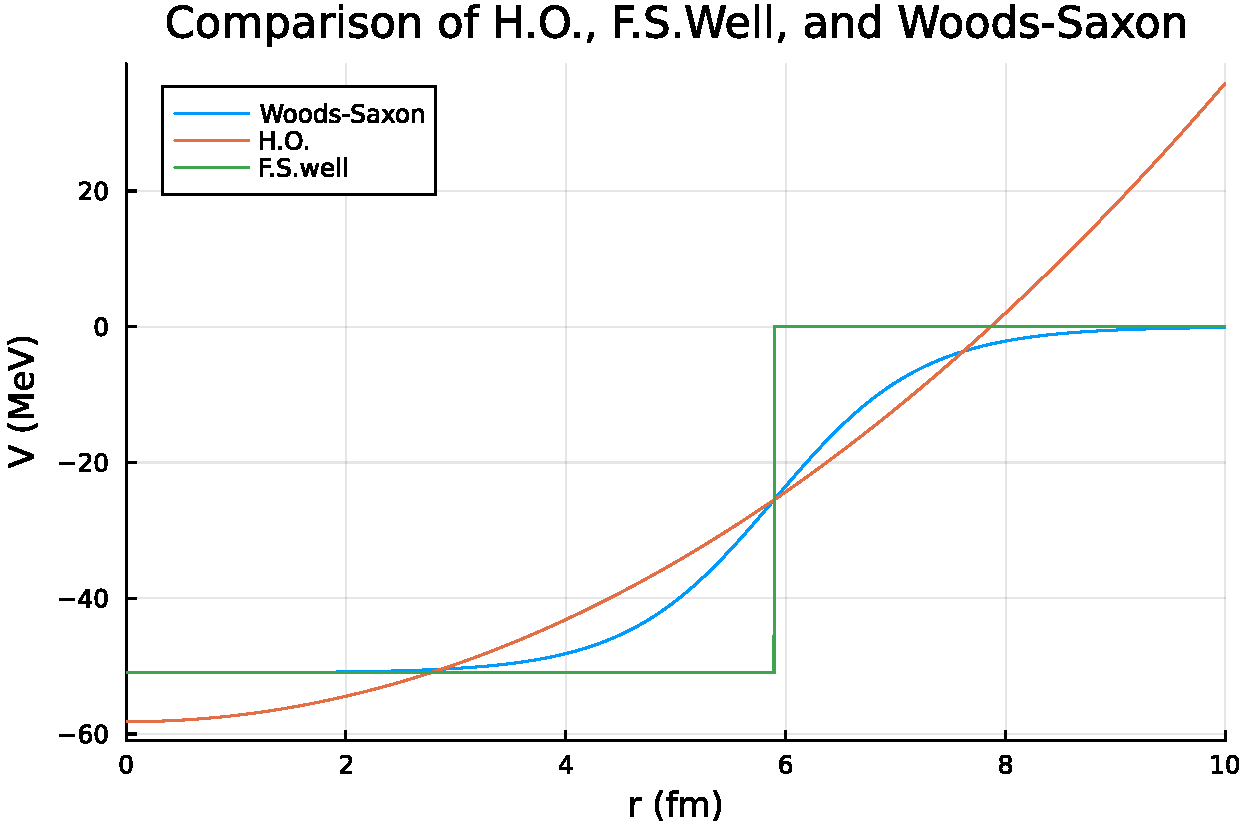
\includegraphics[width=0.8\textwidth]{main_fig/Comp_pt.pdf}
    \caption{3種類のポテンシャルの比較。\\
    凡例の上からWood-Saxon型、調和振動子型、有限井戸型。}
    \label{potential}
  \end{figure}
  %Woods-Saxonポテンシャルを用いれば調和振動子型では縮退していた異なる\(\ell\)の縮退が解ける(図())。  後で入れる。
  \section{seniorityペアリングモデルと対相関}
  % 対相関とは陽子-陽子、中性子-中性子間に働く短距離力によるものであり、一般に対相関を取り込んだHamiltonianは、
  % \begin{equation}
  %   H=\sum_{i}\epsilon_i N_i - \sum_{ij>0}G_{ij} a^{\dagger}_{i}a^{\dagger}_{\bar{i}}a_{\bar{j}}a_{j}
  % \end{equation}
  % である。特にseniorityペアリングでは角運動量の和が0になるような(\(m,-m\))ペアの間で働き、ペアリングの強さを表す\(G\)はその場合のみ値を持つようになるため、
  % 基準に単粒子エネルギーのみの場合を採用すればHamiltonianの形は、
  % \begin{equation}
  %   H=-G\sum_{m,m'>0}a^{\dagger}_{m'}a^{\dagger}_{-m'}a_{-m}a_{m}=-GS_{+}S_{-}.
  % \end{equation}
  % ここで、
  % \begin{equation}
  %   S_{+}=\sum_{m>0}a^{\dagger}_{m}a^{\dagger}_{-m};\quad S_{-}=(S_{+})^{\dagger}\label{quasi-spin}
  % \end{equation}
  % (\ref{quasi-spin})中の\(S_{+},S_{-}\)は擬スピン昇降演算子と呼ばれ、擬スピン演算子はそれぞれのsubstate \(m\)に対して、
  % \begin{align}
  %   s^{(m)}_+ &= a^{\dagger}_{m}a^{\dagger}_{-m}\\
  %   s^{(m)}_- &= a_{-m}a_{m}\\
  %   s^{(m)}_0 &= \frac{1}{2}\left(a^{\dagger}_{m}a_{m}+a^{\dagger}_{-m}a_{-m}-1\right)
  % \end{align}
  % と定義される。このとき、\(a^{\dagger}_{m},a_{m}\)の交換関係を用いると、
  % \begin{align}
  %   \comm{s^{(m)}_+}{s^{(m)}_-} &= 2s^{(m)}_0;\\
  %   \comm{s^{(m)}_0}{s^{(m)}_+} &= s^{(m)}_+;\\
  %   \comm{s^{(m)}_0}{s^{(m)}_-} &= -s^{(m)}_-
  % \end{align}
  % と角運動量演算子と同様の交換関係を導くことができる。
  対相関とは、陽子-陽子および中性子-中性子間に働く短距離力によるものであり、一般に、対相関を取り込んだハミルトニアンは、
  \begin{equation}
    H=\sum_{i}\epsilon_i N_i - \sum_{ij>0}G_{ij} a^{\dagger}_{i}a^{\dagger}_{\bar{i}}a_{\bar{j}}a_{j}
  \end{equation}
  である。特にseniorityペアリングでは角運動量の和が0になるような(\(m,-m\))ペアの間で働き、ペアリングの強さを表す\(G\)はその場合のみ値を持つようになるため、
  基準として単粒子エネルギーのみを採用すれば、ハミルトニアンの形は、
  \begin{equation}
    H=-G\sum_{m,m'>0}a^{\dagger}_{m'}a^{\dagger}_{-m'}a_{-m}a_{m}=-GS_{+}S_{-}.
  \end{equation}
  ここで、
  \begin{equation}
    S_{+}=\sum_{m>0}a^{\dagger}_{m}a^{\dagger}_{-m};\quad S_{-}=(S_{+})^{\dagger}\label{quasi-spin}
  \end{equation}
  (\ref{quasi-spin})中の\(S_{+},S_{-}\)は擬スピン昇降演算子と呼ばれ、擬スピン演算子はそれぞれのsubstate \(m\)に対して、
  \begin{align}
    s^{(m)}_+ &= a^{\dagger}_{m}a^{\dagger}_{-m}\\
    s^{(m)}_- &= a_{-m}a_{m}\\
    s^{(m)}_0 &= \frac{1}{2}\left(a^{\dagger}_{m}a_{m}+a^{\dagger}_{-m}a_{-m}-1\right)
  \end{align}
  と定義される。このとき、\(a^{\dagger}_{m}\)と\(a_{m}\)の交換関係を用いると、
  \begin{align}
    \comm{s^{(m)}_+}{s^{(m)}_-} &= 2s^{(m)}_0;\\
    \comm{s^{(m)}_0}{s^{(m)}_+} &= s^{(m)}_+;\\
    \comm{s^{(m)}_0}{s^{(m)}_-} &= -s^{(m)}_-
  \end{align}
  と角運動量演算子と同様の交換関係を導くことができる。

  % \section{BCS理論}
  % 1957年にBardeen, Cooper, Schriefferによって電子対の考えを基礎にし超伝導を説明する
  % BCS理論が提唱された。この理論によって得られるBCS基底状態、
  % \begin{equation}
  %   \BCSket=\prod_{k>0}\left(u_k + v_k a^{\dagger}_ka^{\dagger}_{\bar{k}}\right)\ket{0}
  % \end{equation}
  % を基底状態として採用する。ここで\(u_k,v_k\)は変分パラメータで、
  % \begin{equation}
  %   \abs{u_k}^2+\abs{v_k}^2=1;\quad u_k>0\label{rest}
  % \end{equation}
  % の条件を満たす。\par
  % 多体系のHamiltonianを単粒子エネルギーの行列表示\(t_{k_1k_2}\)と反対称化された二体相互作用の行列要素\(\bar{v}_{k_1k_2k_3k_4}\)
  % の2つを用いて表すと、
  % \begin{equation}
  %   H=\sum_{k_1 k_2 \lessgtr  0}t_{k_1 k_2} a^{\dagger}_{k_1}a_{k_2}+
  %   \dfrac{1}{4}\sum_{k_1k_2k_3k_4\lessgtr0}\bar{v}_{k_1k_2k_3k_4}a^{\dagger}_{k_1}a^{\dagger}_{k_2}a_{k_4}a_{k_3}
  % \end{equation}
  % と表される。これを元に以下の議論を求めていく。
  % 重要な方程式として粒子数を保存するという条件を課すことで得られる、
  % \begin{equation}
  %   \BCSbra \hat{N} \BCSket =2 \sum_{k>0} v_k^2 = N\label{number}
  % \end{equation}
  % を用いる。この式を用いてHamiltonianに化学ポテンシャル\(\lambda\)と個数演算子\(\hat{N}\)を用いて計算した、
  % \begin{equation}
  %   H'=H-\lambda \hat{N}
  % \end{equation}
  % を使って計算していく。エネルギー期待値は、
  % \begin{equation}
  %   \BCSexp{H'} =\sum_{k\lessgtr0}\left\{(t_{kk}-\lambda)v_{k}^2 +\frac{1}{2}\sum_{k'\lessgtr0}\bar{v}_{kk'kk'}v_{k}^2v_{k'}^2  \right\}
  %     +\sum_{kk'>0}\bar{v}_{k\bar{k}k'\bar{k'}}u_kv_ku_{k'}v_{k'}
  % \end{equation}
  % と導かれる。これを最小にするように変分原理を用いてパラメータ\(\{u_k,v_k\}\)を決定する。
  % \begin{equation}
  %   \delta\BCSexp{H'}=0
  % \end{equation}
  % を計算すると最後にBCS方程式として、
  % \begin{align}
  %   2\tilde{\epsilon}_ku_kv_k+\Delta_k(v_k^2-u_k^2)=0,\quad k>0\label{BCS1} \\
  %   \tilde{\epsilon}_k=\frac{1}{2}\left(t_{kk}+t_{\bar{k}\bar{k}}+\sum_{k'\lessgtr0}(\bar{v}_{kk'kk'}+\bar{v}_{\bar{k}k'\bar{k}k'})v_{k'}^2\right)-\lambda\\
  %   \Delta_k=-\sum_{k'>0}\bar{v}_{k\bar{k}k'\bar{k'}}u_{k'}v_{k'}\label{Delta1}
  % \end{align}
  % が得られる。また、(\ref{rest}),(\ref{BCS1})から\(\tilde{\epsilon}_k,\Delta_k\)を固定した時の\(\{u_k,v_k\}\)の形式解は、
  % \begin{align}
  %   v_k^2&=\frac{1}{2}\left[
  %     1\pm\dfrac{\tilde{\epsilon}_k}{\sqrt{\tilde{\epsilon}_k^2+\Delta_k^2}}
  %   \right]\\
  %   u_k^2&=\frac{1}{2}\left[
  %     1\pm\dfrac{\tilde{\epsilon}_k}{\sqrt{\tilde{\epsilon}_k^2+\Delta_k^2}}
  %   \right]
  % \end{align}
  % と導くことができる。pairingがない場合を考えると、
  % \(\Delta=0\)の時の値は占有されている軌道(\(\tilde{\epsilon}_k<0\))において、\(v_k^2=1,u_k^2=0\)となるように符号を選べばよいので、
  % \begin{align}
  %   v_k^2&=\frac{1}{2}\left[
  %     1-\dfrac{\tilde{\epsilon}_k}{\sqrt{\tilde{\epsilon}_k^2+\Delta_k^2}}
  %   \right]\\
  %   u_k^2&=\frac{1}{2}\left[
  %     1+\dfrac{\tilde{\epsilon}_k}{\sqrt{\tilde{\epsilon}_k^2+\Delta_k^2}}
  %   \right]
  % \end{align}
  % となる。\par
  % seniorityペアリングモデルを適用したとき、単粒子エネルギーの行列表示や二体相互作用作用の行列要素が簡単になる
  % \begin{equation}
  %   t_{k}=t_{\bar{k}}=\epsilon_k,\bar{v}_{k_1k_2k_3k_4}=-G.
  % \end{equation}
  % そのため、Hamiltonian \(H\)の形も変わり、
  % \begin{equation}
  %   H=\sum_{k>0}\epsilon_k(a^{\dagger}_ka_k+a^{\dagger}_{\bar{k}}a_{\bar{k}})-G\sum_{kk'>0}a^{\dagger}_ka^{\dagger}_{\bar{k}}a_{\bar{k'}}a_{k'}\label{Hamiltonian1}
  % \end{equation}
  % となる。同様にエネルギー期待値も変化し、
  % \begin{equation}
  %   \BCSexp{H'}=2\sum_{k>0}\left(\tilde{\epsilon}_kv_k^2+\frac{1}{2}Gv_k^4\right)-\frac{\Delta^2}{G}
  % \end{equation}
  % と計算することができ、\(\tilde{\epsilon}_k\)は、
  % \begin{equation}
  %   \tilde{\epsilon}_k=\epsilon_k -\lambda - Gv_k^2
  % \end{equation}
  % である。
  % \(Gv_k^2,Gv_k^4\)は今回重要ではないため無視する。
  % また\(\Delta\)が\(k\)に依存しなくなるため\(\{u_k,v_k\}\)は、
  % \begin{equation}
  %   \left.\begin{aligned}
  %     u_k^2\\
  %     v_k^2
  %   \end{aligned}\right\}=
  %   \frac{1}{2}\left[
  %     1\pm\frac{\epsilon_k - \lambda}{\sqrt{(\epsilon_k-\lambda)^2+\Delta^2}}
  %   \right]
  % \end{equation}
  % となっている。
  % その場合の粒子数保存の条件、gap方程式は、
  % \begin{align}
  %   N       &=  2\sum_{k>0}v_k^2 \label{number1}\\
  %   \Delta  &=  \dfrac{G}{2}\sum_{k>0}\dfrac{\Delta}{\sqrt{(\epsilon_k-\lambda)^2+\Delta^2}}\label{Delta2}
  % \end{align}
  % のようになり、この2式を数値計算で用いる。
  \section{BCS理論}
  1957年にBardeen, Cooper, Schriefferによって電子対の概念を基礎にして超伝導を説明するBCS理論が提唱された。
  この理論では、時間反転演算子\(T\)を用いて、BCS基底状態
  \begin{equation}
      \BCSket=\prod_{k>0}\left(u_k + v_k a^{\dagger}_ka^{\dagger}_{\bar{k}}\right)\ket{0};\quad\ket{\bar{k}}=T\ket{k}
  \end{equation}
  を基底状態として採用する。ここで、\(u_k,v_k\)は変分パラメータであり、
  \begin{equation}
      \abs{u_k}^2+\abs{v_k}^2=1, \quad u_k>0\label{rest}
  \end{equation}
  の条件を満たす。
  時間反転状態とは、\(\ket{k}=\ket{n\ell j m}\)のとき、\(\ket{\bar{k}}=\ket{n\ell j -m}\)が例である。
  電子対を記述する理論であるため、
  これが核子のpairingについても記述できるとして原子核に適用する。
  \par
  多体系のHamiltonianを単粒子エネルギーの行列要素\(t_{k_1k_2}\)と、反対称化された二体相互作用の行列要素\(\bar{v}_{k_1k_2k_3k_4}\)を用いて表すと、
  \begin{equation}
      H=\sum_{k_1 k_2 \lessgtr  0}t_{k_1 k_2} a^{\dagger}_{k_1}a_{k_2}+
      \dfrac{1}{4}\sum_{k_1k_2k_3k_4\lessgtr0}\bar{v}_{k_1k_2k_3k_4}a^{\dagger}_{k_1}a^{\dagger}_{k_2}a_{k_4}a_{k_3}
  \end{equation}
  と表される。これを基に以下の議論を進める。\par
  重要な方程式として、粒子数保存の条件から得られる
  \begin{equation}
      \BCSbra \hat{N} \BCSket =2 \sum_{k>0} v_k^2 = N\label{number}
  \end{equation}
  を用いる。この式を基に、Hamiltonianに化学ポテンシャル\(\lambda\)と粒子数演算子\(\hat{N}\)を導入し、
  \begin{equation}
      H'=H-\lambda \hat{N}
  \end{equation}
  と定義する。\par
  エネルギー期待値は
  \begin{equation}
      \BCSexp{H'} =\sum_{k\lessgtr0}\left\{(t_{kk}-\lambda)v_{k}^2 +\frac{1}{2}\sum_{k'\lessgtr0}\bar{v}_{kk'kk'}v_{k}^2v_{k'}^2  \right\}
        +\sum_{kk'>0}\bar{v}_{k\bar{k}k'\bar{k'}}u_kv_ku_{k'}v_{k'}
  \end{equation}
  と計算される。これを最小化するため、変分原理を用いてパラメータ\(\{u_k,v_k\}\)を決定する。
  \begin{equation}
      \delta\BCSexp{H'}=0
  \end{equation}
  を計算すると、最終的にBCS方程式として
  \begin{align}
      2\tilde{\epsilon}_ku_kv_k+\Delta_k(v_k^2-u_k^2)=0, \quad k>0\label{BCS1} \\
      \tilde{\epsilon}_k=\frac{1}{2}\left(t_{kk}+t_{\bar{k}\bar{k}}+\sum_{k'\lessgtr0}(\bar{v}_{kk'kk'}+\bar{v}_{\bar{k}k'\bar{k}k'})v_{k'}^2\right)-\lambda\\
      \Delta_k=-\sum_{k'>0}\bar{v}_{k\bar{k}k'\bar{k'}}u_{k'}v_{k'}\label{Delta1}
  \end{align}
  が得られる。\par
  また、(\ref{rest}), (\ref{BCS1})から、\(\tilde{\epsilon}_k, \Delta_k\)が固定された場合の\(\{u_k,v_k\}\)の形式解は
  \begin{align}
      v_k^2&=\frac{1}{2}\left[
        1\pm\dfrac{\tilde{\epsilon}_k}{\sqrt{\tilde{\epsilon}_k^2+\Delta_k^2}}
      \right]\\
      u_k^2&=\frac{1}{2}\left[
        1\pm\dfrac{\tilde{\epsilon}_k}{\sqrt{\tilde{\epsilon}_k^2+\Delta_k^2}}
      \right]
  \end{align}
  と導かれる。pairingがない場合、すなわち\(\Delta=0\)のとき、占有されている軌道(\(\tilde{\epsilon}_k<0\))では\(v_k^2=1, u_k^2=0\)となるように符号を選ぶと、
  \begin{align}
      v_k^2&=\frac{1}{2}\left[
        1-\dfrac{\tilde{\epsilon}_k}{\sqrt{\tilde{\epsilon}_k^2+\Delta_k^2}}
      \right]\\
      u_k^2&=\frac{1}{2}\left[
        1+\dfrac{\tilde{\epsilon}_k}{\sqrt{\tilde{\epsilon}_k^2+\Delta_k^2}}
      \right]
  \end{align}
  となる。\par
  seniorityペアリングモデルを適用すると、単粒子エネルギーの行列要素や二体相互作用の行列要素が簡単化され、
  \begin{equation}
      t_{k}=t_{\bar{k}}=\epsilon_k, \quad \bar{v}_{k_1k_2k_3k_4}=-G.
  \end{equation}
  したがって、Hamiltonian \(H\)の形は
  \begin{equation}
      H=\sum_{k>0}\epsilon_k(a^{\dagger}_ka_k+a^{\dagger}_{\bar{k}}a_{\bar{k}})-G\sum_{kk'>0}a^{\dagger}_ka^{\dagger}_{\bar{k}}a_{\bar{k'}}a_{k'}\label{Hamiltonian1}
  \end{equation}
  となる。\par
  同様にエネルギー期待値は
  \begin{equation}
      \BCSexp{H'}=2\sum_{k>0}\left(\tilde{\epsilon}_kv_k^2+\frac{1}{2}Gv_k^4\right)-\frac{\Delta^2}{G}
  \end{equation}
  と計算され、\(\tilde{\epsilon}_k\)は
  \begin{equation}
      \tilde{\epsilon}_k=\epsilon_k -\lambda - Gv_k^2
  \end{equation}
  である。\par
  \(Gv_k^2, Gv_k^4\)は今回重要でないため無視する。また\(\Delta\)が\(k\)に依存しなくなるため\(\{u_k,v_k\}\)は
  \begin{equation}
      \left.\begin{aligned}
        u_k^2\\
        v_k^2
      \end{aligned}\right\}=
      \frac{1}{2}\left[
        1\pm\frac{\epsilon_k - \lambda}{\sqrt{(\epsilon_k-\lambda)^2+\Delta^2}}
      \right]
  \end{equation}
  と表される。\par
  この場合の粒子数保存条件およびgap方程式は
  \begin{align}
      N       &=  2\sum_{k>0}v_k^2 \label{number1}\\
      \Delta  &=  \dfrac{G}{2}\sum_{k>0}\dfrac{\Delta}{\sqrt{(\epsilon_k-\lambda)^2+\Delta^2}}\label{Delta2}
  \end{align}
  のようになり、この2式を数値計算で解く。

  % \section{有限温度BCS理論への拡張}
  % 有限温度では粒子が熱力学的分布に従うため、(\ref{Hamiltonian1})の\(a^{\dagger}_ka_k,a^{\dagger}_{\bar{k}}a_{\bar{k}}\)の期待値に熱力学的分布が含まれる。
  % 同様にgap方程式や粒子数保存の条件も熱力学的分布を含む形に変化する。各方程式の導出は付録\ref{FTBCS導出}に示す。
  % 準粒子エネルギー\(E_k=\sqrt{(\epsilon_k-\lambda)^2+\Delta^2}\),Fermi分布\(f_k=1/(1+e^{\beta E_k})\)を用いて、
  % \begin{align}
  %   \langle a^{\dagger}_ka_k \rangle =\langle a^{\dagger}_{\bar{k}}a_{\bar{k}}\rangle&=
  %   v_k^2(1-f_k)+u_k^2f_k\\
  %   &=\frac{\epsilon_k - \lambda}{2}\left[1-\frac{\epsilon_k-\lambda}{E_k}\tanh(\frac{E_k}{2k_B T})\right]
  % \end{align}
  % となる。Hamiltonianは、
  % \begin{equation}
  %   \langle H'\rangle=\sum_{k>0}(\epsilon_k - \lambda)\left[1-\frac{\epsilon_k-\lambda}{E_k}\tanh(\frac{E_k}{2k_B T})\right]-\frac{\Delta^2}{G}
  % \end{equation}
  % の形に書き直される。
  % 同じようにgap方程式や粒子数保存の条件も修正されて、
  % \begin{align}
  %   N       &= 2\sum_{k>0}\left[v_k^2 + (u_k^2-v_k^2)f_i\right] \notag\\
  %           &= \sum_{k>0}\left(1+\frac{\epsilon_k-\lambda}{\sqrt{(\epsilon_k-\lambda)^2-\Delta^2}}\tanh(\frac{E_k}{2k_BT})\right)\\
  %   \Delta  &= \frac{G}{2}\sum_{k>0}\frac{\Delta}{E_j}\tanh(\frac{E_k}{2k_BT})\label{FTgap}
  % \end{align}
  % のようになる。
  % 式(\ref{FTgap})には自明解\(\Delta=0\)が存在するが、
  % 非自明解が存在する範囲が超流動状態、存在しない範囲が常流動状態と考え温度変化に対する非自明解の応答を見る。
  % 計算方法
  \section{有限温度BCS理論への拡張}
  この章では特に文献(Goodman\cite{goodman1981finite})を参考にした。有限温度では粒子が熱力学的分布に従うため、(\ref{Hamiltonian1})の\(a^{\dagger}_ka_k,a^{\dagger}_{\bar{k}}a_{\bar{k}}\)の期待値に熱力学的分布が含まれる。
  同様にギャップ方程式や粒子数保存条件も熱力学的分布を含む形に変化する。各方程式の導出は付録\ref{FTBCS導出}に示す。以下ではBoltzman定数\(k_B=8.617333\times 10^{-11}\)MeV/K,
  逆温度\(\beta=1/k_B T\)を用いる。
  
  準粒子エネルギー\(E_k=\sqrt{(\epsilon_k-\lambda)^2+\Delta^2}\)、フェルミ分布\(f_k=1/(1+e^{\beta E_k})\)を用いて、
  \begin{align}
    \langle a^{\dagger}_ka_k \rangle =\langle a^{\dagger}_{\bar{k}}a_{\bar{k}}\rangle&=
    v_k^2(1-f_k)+u_k^2f_k\\
    &=\frac{\epsilon_k - \lambda}{2}\left[1-\frac{\epsilon_k-\lambda}{E_k}\tanh(\frac{E_k}{2k_B T})\right]
  \end{align}
  となる。ハミルトニアンは、
  \begin{equation}
    \langle H'\rangle=\sum_{k>0}(\epsilon_k - \lambda)\left[1-\frac{\epsilon_k-\lambda}{E_k}\tanh(\frac{E_k}{2k_B T})\right]-\frac{\Delta^2}{G}
  \end{equation}
  の形に書き直される。
  
  同様にギャップ方程式や粒子数保存条件も修正されて、
  \begin{align}
    N       &= 2\sum_{k>0}\left[v_k^2 + (u_k^2-v_k^2)f_k\right] \notag\\
            &= \sum_{k>0}\left(1+\frac{\epsilon_k-\lambda}{\sqrt{(\epsilon_k-\lambda)^2-\Delta^2}}\tanh(\frac{E_k}{2k_BT})\right)\\
    \Delta  &= \frac{G}{2}\sum_{k>0}\frac{\Delta}{E_k}\tanh(\frac{E_k}{2k_BT})\label{FTgap}
  \end{align}
  のようになる。

  式(\ref{FTgap})には自明解\(\Delta=0\)が存在するが、
  非自明解が存在する範囲が超流動状態、存在しない範囲が常流動状態と考え、温度変化に対する非自明解の応答を見る。

\chapter{数値計算方法}
%   \section{単粒子ハミルトニアンの対角化}
%   単粒子HamiltonianはWoods-Saxonポテンシャルとスピン軌道相互作用を採用し、
%   \begin{equation}
%     H=T_{\text{H.O.}}+U(r)
%   \end{equation}
%   のように定義される。ここで\(T_{\text{H.O.}}\)は調和振動子のエネルギー固有値であり、
%   具体的な形は、
%   \begin{equation}
%     T_{\text{H.O.}} = \hbar\omega\left(2n+\ell+\frac{3}{2}\right);\quad\hbar\omega=41A^{-1/3}.
%   \end{equation}
%   ポテンシャル項\(U(r)\)は、
%   \begin{equation}
%     U(r) = u_0 f(r) + u_{ls} r_0^2 \frac{1}{r} \frac{df(r)}{dr} \boldsymbol{l} \cdot \boldsymbol{s}
%       + U_{\text{Coul}}(r) \frac{1 - \tau}{2}-\frac{1}{2}M\omega^2r^2;\quad f(r)=\frac{1}{1 + \exp \left( \frac{r - R}{a} \right)}.
%   \end{equation}
%   この時のポテンシャルパラメータは、以下の表にまとめた。\par
%   \begin{table}[htbp]
%     \centering
%     \caption{ポテンシャルパラメータの一覧}
%     \begin{tabular}{c c c c}
%         \hline
%         記号 & 値 & 単位 & 備考 \\
%         \hline
%         \( u_0 \) & \(-51+33(N-Z)/A\) & MeV & ポテンシャルの深さ \\
%         \( u_{ls} \) & \(22-14(N-Z/A)\) & MeV & スピン軌道相互作用の強さ \\
%         \(r_0\)    & 1.27              &  fm & 長さの基準\\
%         \( R \) & \(r_0 A^{1/3}\) & fm & 原子核半径 \\
%         \( a \) & 0.67 & fm & 原子核の広がり \\
%         \hline
%     \end{tabular}
% \end{table}
%   このHamiltonianを極座標調和振動子基底とスピン波動関数の直積によって表現される展開し、対角化を行うことで単粒子エネルギーを求めた。
%   波動関数は以下に示すとおりである。
%   \begin{align}
%     \psi_{nm\ell j}(r)  &=\frac{u_{n\ell}(q)}{r}\mathcal{Y}_{\ell j m}(\theta,\phi)\\
%     u_{n\ell}(q)        &=\sqrt{2a\dfrac{\varGamma(\ell+n+3/2)}{n!(\varGamma^2(\ell+3/2))}}q^{\ell+1}e^{-q^2/2}M(-n,\ell+3/2,q^2)\\
%     \mathcal{Y}_{\ell j m}(\theta,\phi)
%     &=\pm\sqrt{\frac{\ell \pm m + 1/2}{2\ell+1}}Y_{\ell m-1/2}(\theta,\phi)\ket{+}+\sqrt{\frac{\ell \mp m + 1/2}{2\ell+1}}Y_{\ell m+1/2}(\theta,\phi)\ket{-}
%   \end{align}
%   ここで、\(Y_{\ell m}(\theta,\phi)\)は球面調和関数、\(\Gamma(n)\)はガンマ関数、\(M(\beta,\gamma,x)\)は合流型超幾何関数、\(q=ar,a=\sqrt{\frac{M\omega}{\hbar}}\)である。
  \section{単粒子ハミルトニアンの対角化}
  単粒子HamiltonianはWoods-Saxonポテンシャルとスピン軌道相互作用を採用し、
  \begin{equation}
    H=T_{\text{H.O.}}+U(r)
  \end{equation}
  のように定義される。ここで\(T_{\text{H.O.}}\)は調和振動子のエネルギー固有値であり、
  具体的な形は、
  \begin{equation}
    T_{\text{H.O.}} = \hbar\omega\left(2n+\ell+\frac{3}{2}\right),\quad \hbar\omega=41A^{-1/3}.
  \end{equation}
  ポテンシャル項\(U(r)\)は、
  \begin{equation}
    U(r) = u_0 f(r) + u_{ls} r_0^2 \frac{1}{r} \frac{df(r)}{dr} \boldsymbol{l} \cdot \boldsymbol{s}
      + U_{\text{Coul}}(r) \frac{1 - \tau}{2}-\frac{1}{2}M\omega^2r^2, \quad f(r)=\frac{1}{1 + \exp \left( \frac{r - R}{a} \right)}.
  \end{equation}
  この時のポテンシャルパラメータは、\(N,Z,A\)をそれぞれ中性子数、陽子数、核子数として以下の表にまとめた。\par
  \begin{table}[htbp]
    \centering
    \caption{ポテンシャルパラメータの一覧}
    \begin{tabular}{c c c c}
        \hline
        記号 & 値 & 単位 & 備考 \\
        \hline
        \( u_0 \) & \(-51+33(N-Z)/A\) & MeV & ポテンシャルの深さ \\
        \( u_{ls} \) & \(22-14(N-Z)/A\) & MeV & スピン軌道相互作用の強さ \\
        \(r_0\)    & 1.27              &  fm & 長さの基準\\
        \( R \) & \(r_0 A^{1/3}\) & fm & 原子核半径 \\
        \( a \) & 0.67 & fm & 原子核の広がり \\
        \hline
    \end{tabular}
  \end{table}

  このHamiltonianを極座標調和振動子基底とスピン波動関数の直積によって展開し、対角化を行うことで単粒子エネルギーを求めた。
  波動関数は以下に示すとおりである。
  \begin{align}
    \psi_{nm\ell j}(r)  &=\frac{u_{n\ell}(q)}{r}\mathcal{Y}_{\ell j m}(\theta,\phi),\\
    u_{n\ell}(q)        &=\sqrt{2a\dfrac{\Gamma(\ell+n+3/2)}{n!(\Gamma^2(\ell+3/2))}}q^{\ell+1}e^{-q^2/2}M(-n,\ell+3/2,q^2),\\
    \mathcal{Y}_{\ell j m}(\theta,\phi)
    &=\pm\sqrt{\frac{\ell \pm m + 1/2}{2\ell+1}}Y_{\ell, m-1/2}(\theta,\phi)\ket{+}
    +\sqrt{\frac{\ell \mp m + 1/2}{2\ell+1}}Y_{\ell, m+1/2}(\theta,\phi)\ket{-}.
  \end{align}
  ここで、\(Y_{\ell m}(\theta,\phi)\)は球面調和関数、\(\Gamma(n)\)はガンマ関数、\(M(\beta,\gamma,x)\)は合流型超幾何関数、
  \(q=ar\), \(a=\sqrt{\frac{M\omega}{\hbar}}\) である。

  % \section{ペアリング強度・化学ポテンシャルの計算}
  % 以降はmodel spaceとして魔法数の50と82の間の軌道の、\(0g_{7/2},1d_{5/2},1d_{3/2},2s_{1/2},0h_{11/2}\)を取り計算を行う。
  % 初期値として、ギャップパラメータは文献\cite{thenuclearmanybody}より、\(\Delta=12\cdot A^{-1/2}\)
  % を採用し、化学ポテンシャル\(\lambda\)はその値を用いて粒子数保存の条件
  % \begin{equation}
  %   N=\sum_{k>0}\left(1-\frac{\epsilon_k - \lambda}{\sqrt{(\epsilon_k-\lambda)^2}+\Delta^2}\right) \label{number2}
  % \end{equation}
  % を数値的に解くことで得る。得られた\(\Delta,\lambda\)を、非自明な解を求めるギャップ方程式、
  % \begin{equation}
  %   1 = \dfrac{G}{2}\sum_{k>0}\dfrac{1}{\sqrt{(\epsilon_k-\lambda)^2+\Delta^2}} \label{Delta3}
  % \end{equation}
  % に代入することでペアリング強度\(G\)を求めた。
  \section{ペアリング強度・化学ポテンシャルの計算}
  以降は、model spaceとして魔法数50と82の間の軌道である\(0g_{7/2},1d_{5/2},1d_{3/2},2s_{1/2},0h_{11/2}\)を用いて計算を行う。

  pairing gap\(\Delta\)は文献(Ring and Schuck\cite{thenuclearmanybody})に基づき
  \(\Delta=12\cdot A^{-1/2}\)を採用し、化学ポテンシャル\(\lambda\)はこの\(\Delta\)を用いて、粒子数保存の条件
  \begin{equation}
    N=\sum_{k>0}\left(1-\frac{\epsilon_k - \lambda}{\sqrt{(\epsilon_k-\lambda)^2+\Delta^2}}\right) \label{number2}
  \end{equation}
  に代入し、$\lambda$が収束するまで計算を行うことで数値的に求める。

  得られた\(\Delta,\lambda\)をギャップ方程式
  \begin{equation}
    1 = \dfrac{G}{2}\sum_{k>0}\dfrac{1}{\sqrt{(\epsilon_k-\lambda)^2+\Delta^2}} \label{Delta3}
  \end{equation}
  に代入することで、ペアリング強度\(G\)を求める。

  % \section{温度依存性の計算手法}
  % 有限温度BCS理論に基づき、温度に上昇に伴う化学ポテンシャル\(\lambda\)およびペアリングギャップ\(\Delta\)の変化を求めた。
  % 温度範囲 $T = 0.0$ 〜 $1.0$ MeV に対して、まず全体を $0.05$ MeV 刻みで計算し、ギャップが急激に変化する領域の特定を行った。  
  % 次に、ギャップの変化が大きい領域(得られた転移温度の $\pm 0.2$ MeV 周辺)では、より細かい $0.005$ MeV 刻みで計算を実施し、相転移点付近の詳細な振る舞いを解析した。
  % ギャップ方程式と粒子数保存の条件の
  % \begin{align}
  %   N       &= \sum_{k>0}\left(1+\frac{\epsilon_k-\lambda}{\sqrt{(\epsilon_k-\lambda)^2-\Delta^2}}\tanh(\frac{E_k}{2k_BT})\right)\\
  %   \Delta  &= \frac{G}{2}\sum_{k>0}\frac{\Delta}{\sqrt{(\epsilon_k-\lambda)^2-\Delta^2}}\tanh(\frac{E_k}{2k_BT})
  % \end{align}
  % を各温度ごとにとき、収束した値を記録した。ここで\(E_k=\sqrt{(\epsilon_k-\lambda)^2-\Delta^2}\).
  % 同様に各温度でのエネルギー期待値、
  % \begin{equation}
  %   \langle H'\rangle=\sum_{k>0}(\epsilon_k - \lambda)\left[1-\frac{\epsilon_k-\lambda}{E_k}\tanh(\frac{E_k}{2k_B T})\right]-\frac{\Delta^2}{G}
  % \end{equation}
  % も求め、これを数値微分することで比熱の温度変化も求めた。
  % \begin{equation}
  %   C=\frac{\partial \langle H'\rangle}{\partial T}
  % \end{equation}
  \section{温度依存性の計算手法}
  有限温度BCS理論に基づき、温度の上昇に伴う化学ポテンシャル\(\lambda\)およびpairing gap\(\Delta\)の変化を求めた。
  ただし、ペアリング強度\(G\)は魔法数から離れた核である\ce{{}^{116}Sn}核のものを採用した。 
  温度範囲 \(k_B T = 0.0\) 〜 \(1.0\) MeV に対して、まず全体を \(0.05\) MeV 刻みで計算し、gapが急激に変化する領域を特定した。  
  次に、\(\Delta\)の変化が大きい領域(得られた転移温度の \(\pm 0.2\) MeV 周辺)では、より細かい \(0.005\) MeV 刻みで計算を実施し、相転移点付近の詳細な振る舞いを解析した。  

  ギャップ方程式と粒子数保存の条件  
  \begin{align}
      N &= \sum_{k>0} \left( 1 + \frac{\epsilon_k - \lambda}{\sqrt{(\epsilon_k - \lambda)^2 - \Delta^2}} \tanh \left(\frac{E_k}{2k_B T} \right) \right), \\
      \Delta &= \frac{G}{2} \sum_{k>0} \frac{\Delta}{\sqrt{(\epsilon_k - \lambda)^2 - \Delta^2}} \tanh \left(\frac{E_k}{2k_B T} \right)
  \end{align}
  を各温度ごとに解き、収束した値を記録した。  
  ここで \(E_k = \sqrt{(\epsilon_k - \lambda)^2 - \Delta^2}\) である。  

  同様に、各温度でのエネルギー期待値  
  \begin{equation}
      \langle H' \rangle = \sum_{k>0} (\epsilon_k - \lambda) \left[ 1 - \frac{\epsilon_k - \lambda}{E_k} \tanh \left( \frac{E_k}{2k_B T} \right) \right] - \frac{\Delta^2}{G}
  \end{equation}
  を求め、これを数値微分することで比熱の温度変化を導出した。  
  \begin{equation}
      C = \frac{\partial \langle H' \rangle}{\partial T}
  \end{equation}

% 結果と考察
\chapter{結果と考察}
  ここでは数値計算の結果を示す。
  また、ペアリング相関と相転移の関連について関心があるため、
  計算対象の原子核から\ce{{}^{100}Sn},\ce{{}^{132}Sn}を排した。
  \section{ペアリング強度、化学ポテンシャルの核子数依存性}
  \(T=0\)Kの場合のペアリング強度\(G\)と化学ポテンシャル\(\lambda\)の計算結果を示す。
  ペアリング強度の計算結果に添えた近似式\(G=22/A\)は文献(Baranger and Kumar\cite{baranger1968nuclear})から利用した。
  \begin{figure}[H]
    \centering
    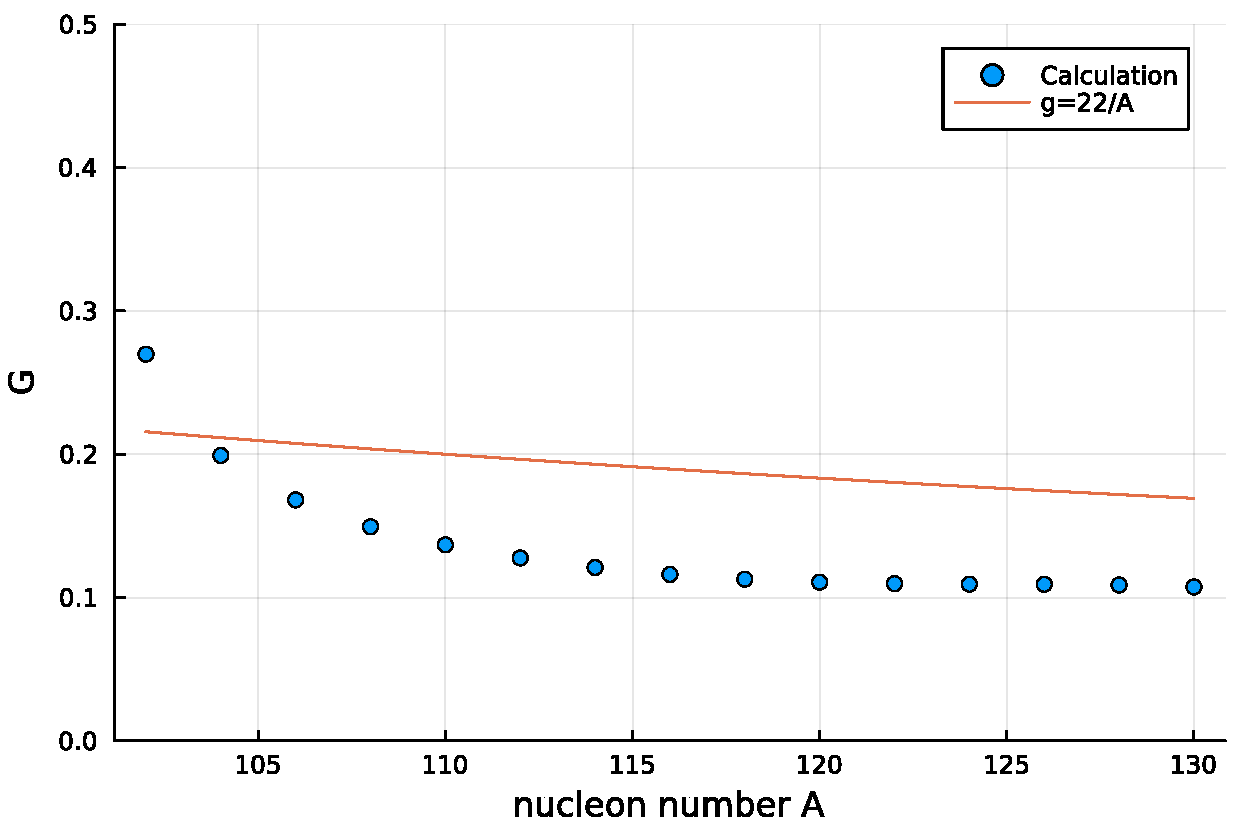
\includegraphics[width=0.8\textwidth]{main_fig/G_vs_A.pdf}
    \caption{核子数依存したペアリング強度$G$の計算結果($T=0$\,K)。近似式$G=22/A$は文献(Baranger and Kumar~\cite{baranger1968nuclear})から引用した。}
  \end{figure}
  \begin{figure}[H]
    \centering
    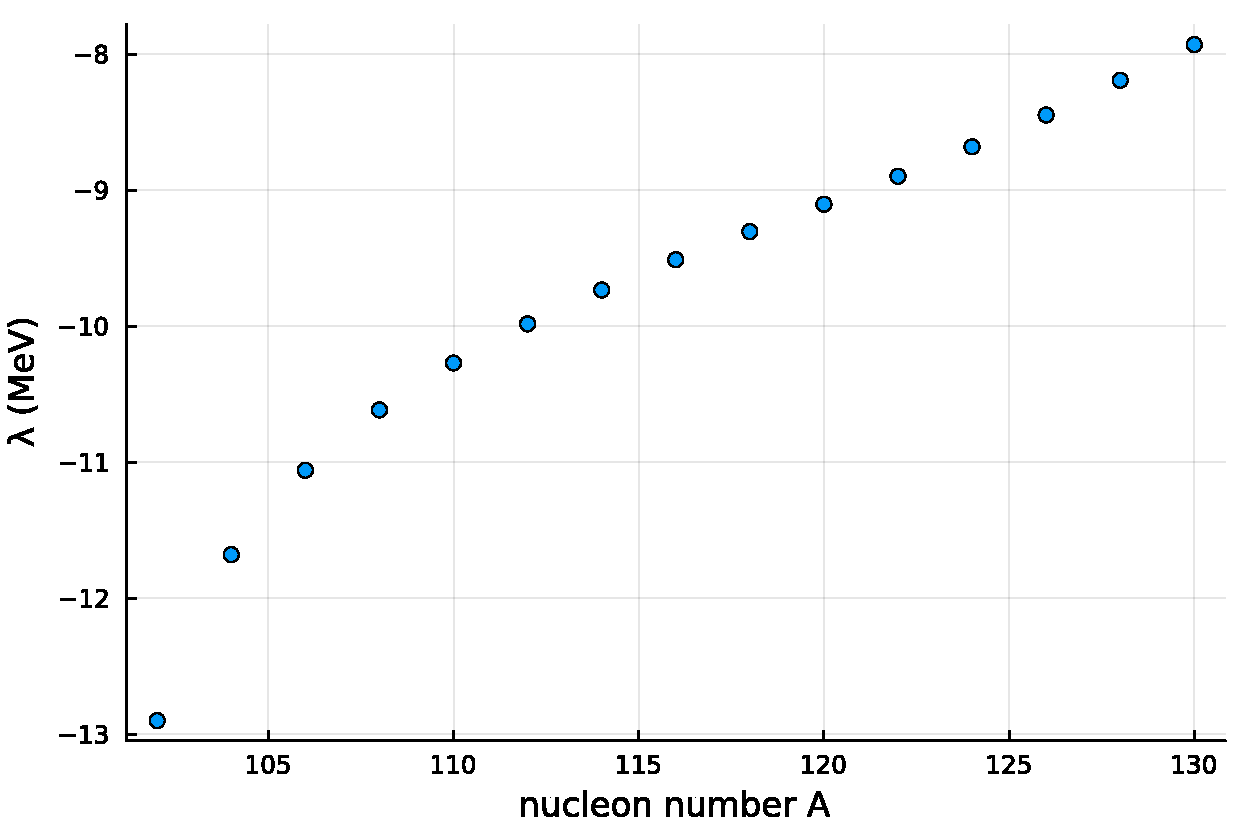
\includegraphics[width=0.8\textwidth]{main_fig/lambda_vs_A.pdf}
    \caption{核子数依存した化学ポテンシャル$\lambda$の計算結果($T=0$\,K)。}
  \end{figure}
  この2つの計算結果から考えられることは、
  \begin{enumerate}
    \item 近似式と比較し、傾向は一致している。
    \item 化学ポテンシャルが核子数に対して単調に増加している。
  \end{enumerate}
  の2点が挙げられる。\par
  1について、
  これはWoods-Saxonポテンシャルとseniorityペアリングモデルの採用することの妥当性を示していると考えられる。\par
  2について、
  化学ポテンシャルが、絶対零度における粒子の存在確率が\(1/2(=\lim_{T\rightarrow0}\frac{1}{\exp((e-\lambda)/k_B T)+1})\)
  になるようなエネルギーを示していることから、妥当であると考える。
  \section{超流動・常流動相転移}
  前節で計算した核子に対応する化学ポテンシャルと、\ce{{}^{116}Sn}のペアリング強度\(G\)を採用した。
  計算結果の表示方法として、視認性を良くするために102~130までを3つにわけることにした。
  pairing gap\(\Delta\)、エネルギー期待値\(\langle H'\rangle\)、比熱\(C\)の温度変化を示し、最後に\(\Delta=0\)になった温度を表とグラフでまとめた。
  $x$軸と$y$軸に表れる\(\Delta_0\)は、\(T=0\)Kでのギャップの値である。
  \begin{figure}[H]
    \centering
    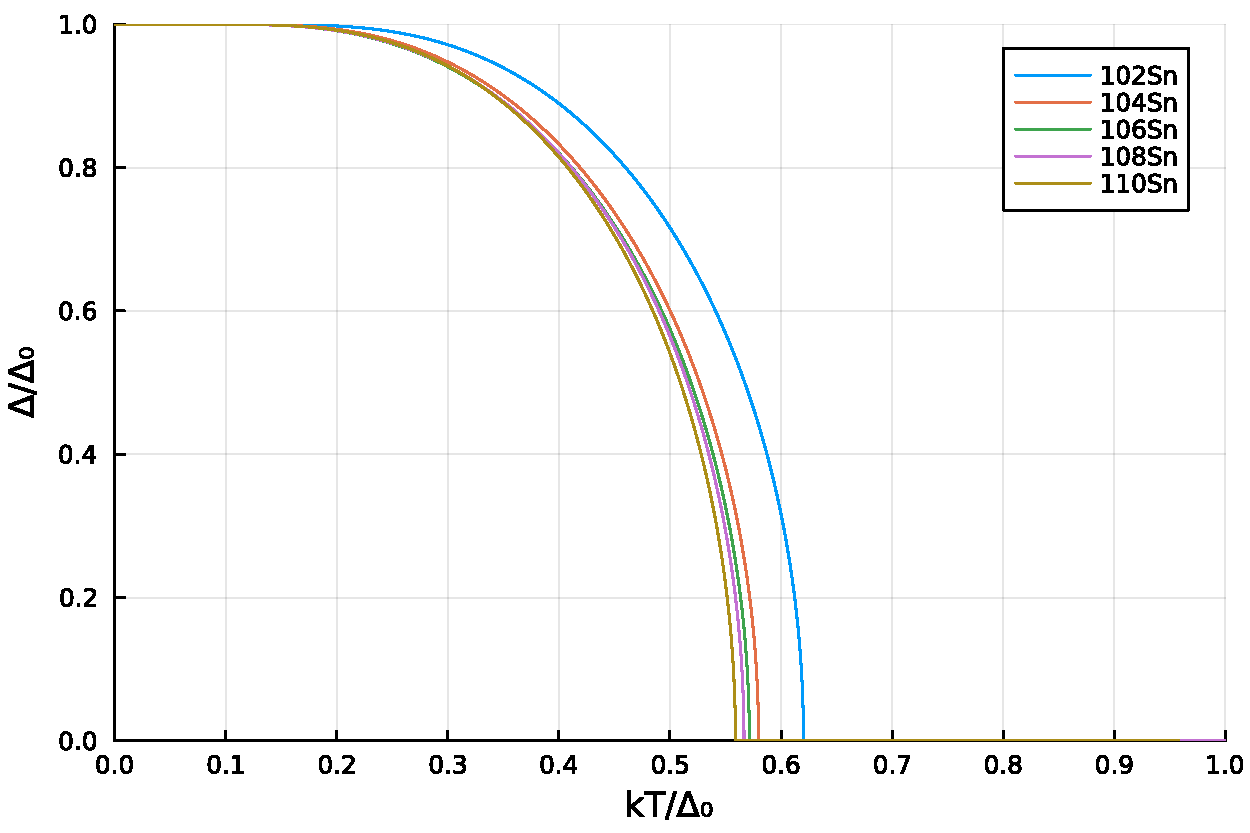
\includegraphics[width=0.65\textwidth]{main_fig/102d.pdf}
    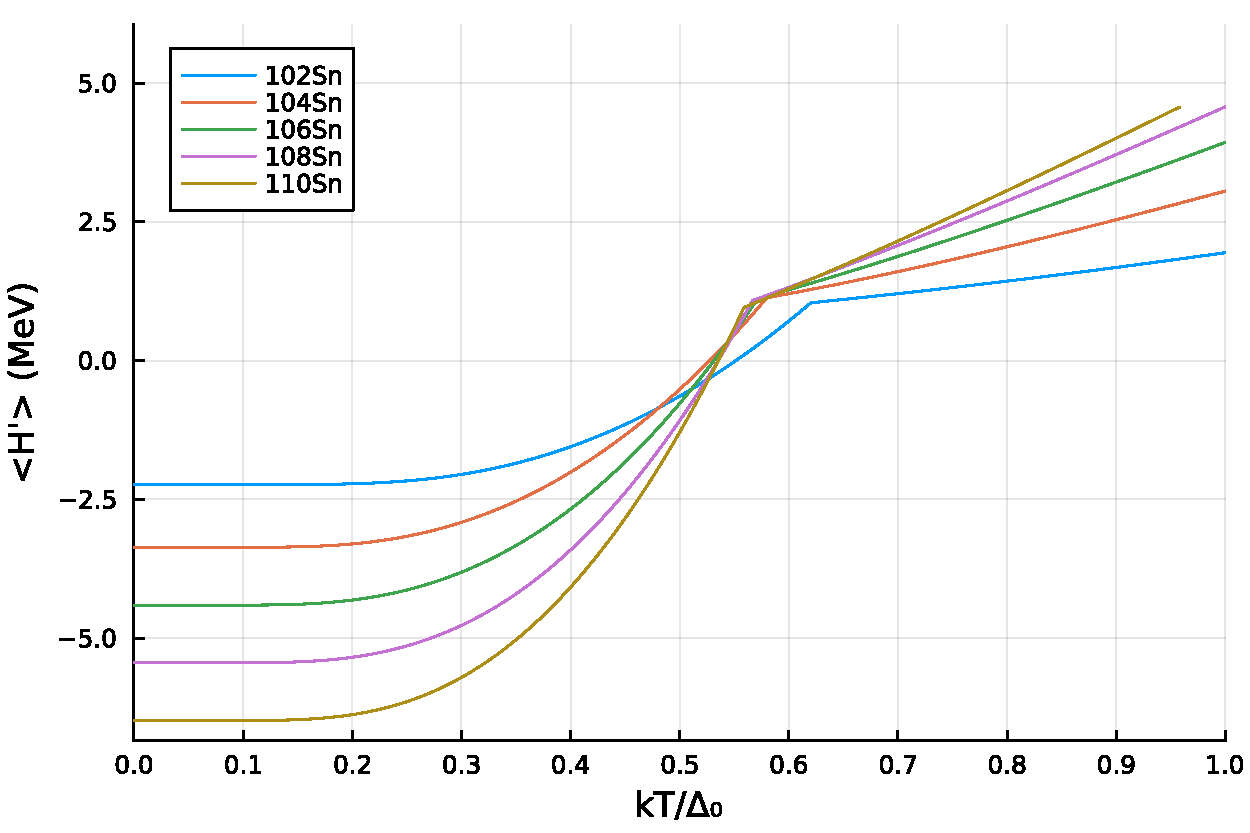
\includegraphics[width=0.65\textwidth]{main_fig/102H.pdf}
    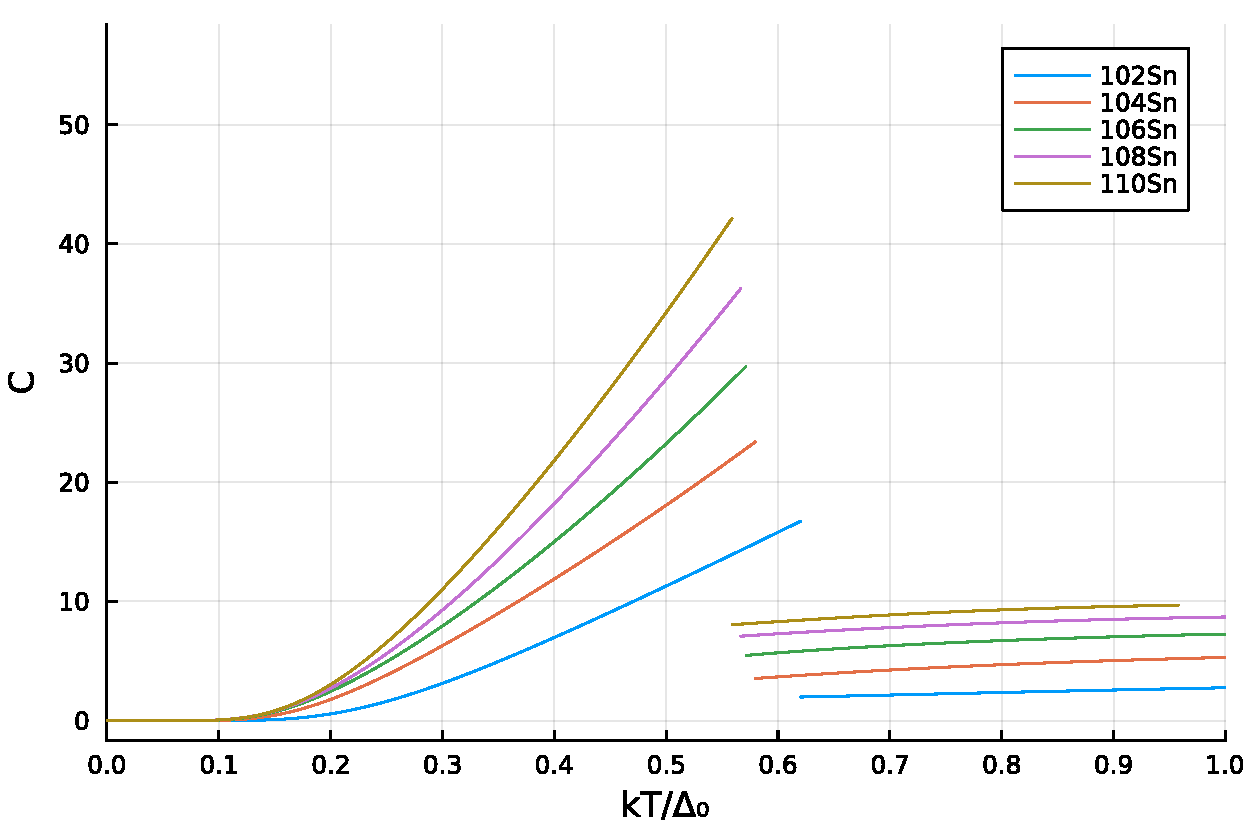
\includegraphics[width=0.65\textwidth]{main_fig/102C.pdf}
    \caption{\ce{{}^{102-110}}Snの中性子についての計算結果。上からpairing gap、エネルギー期待値、比熱に対する温度変化。}
  \end{figure}
  \newpage
  \begin{figure}[H]
    \centering
    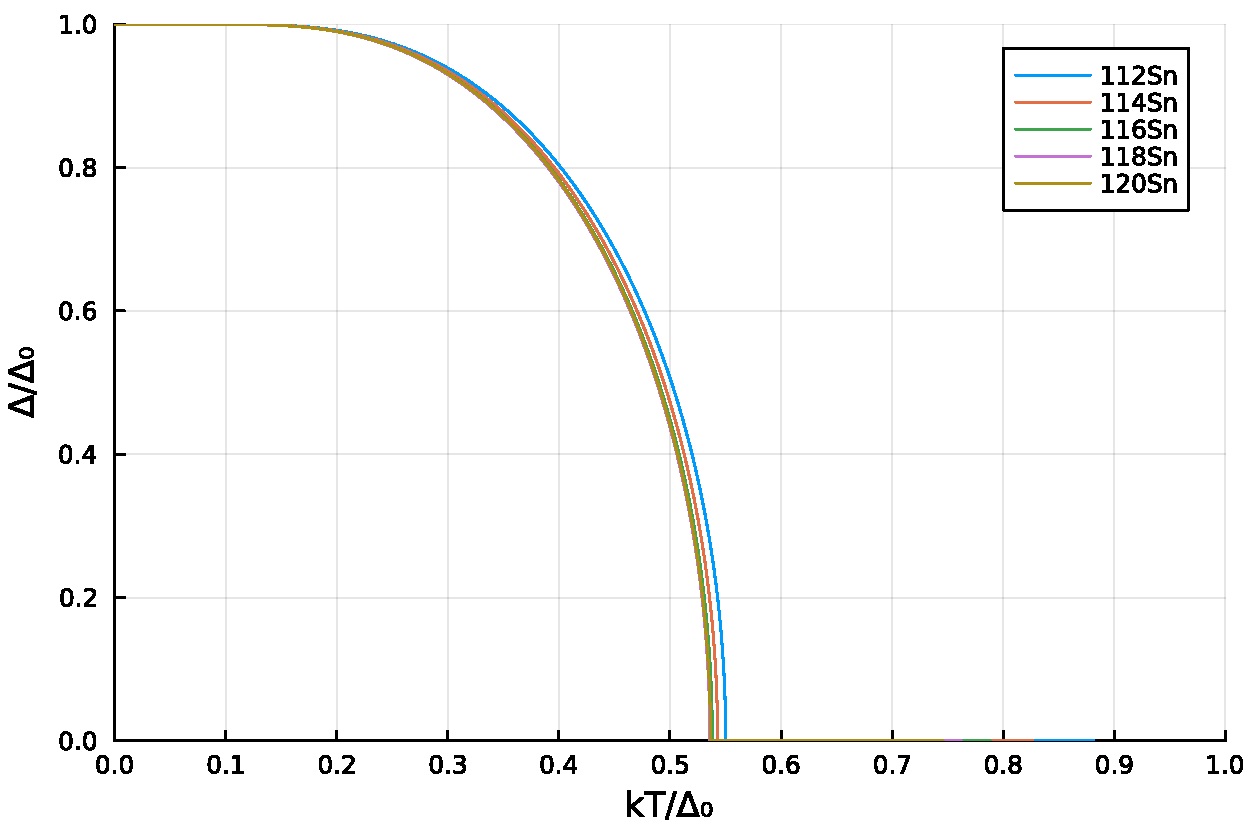
\includegraphics[width=0.65\textwidth]{main_fig/112d.pdf}
    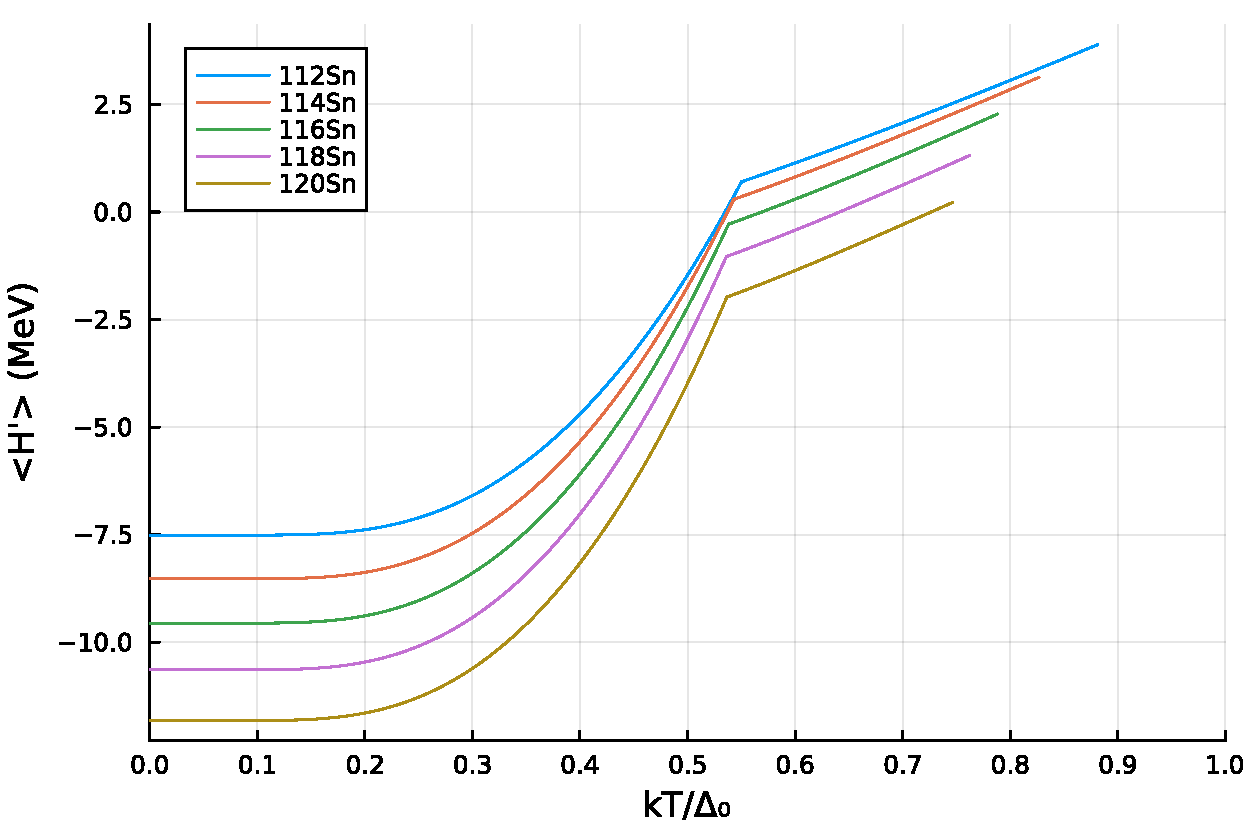
\includegraphics[width=0.65\textwidth]{main_fig/112H.pdf}
    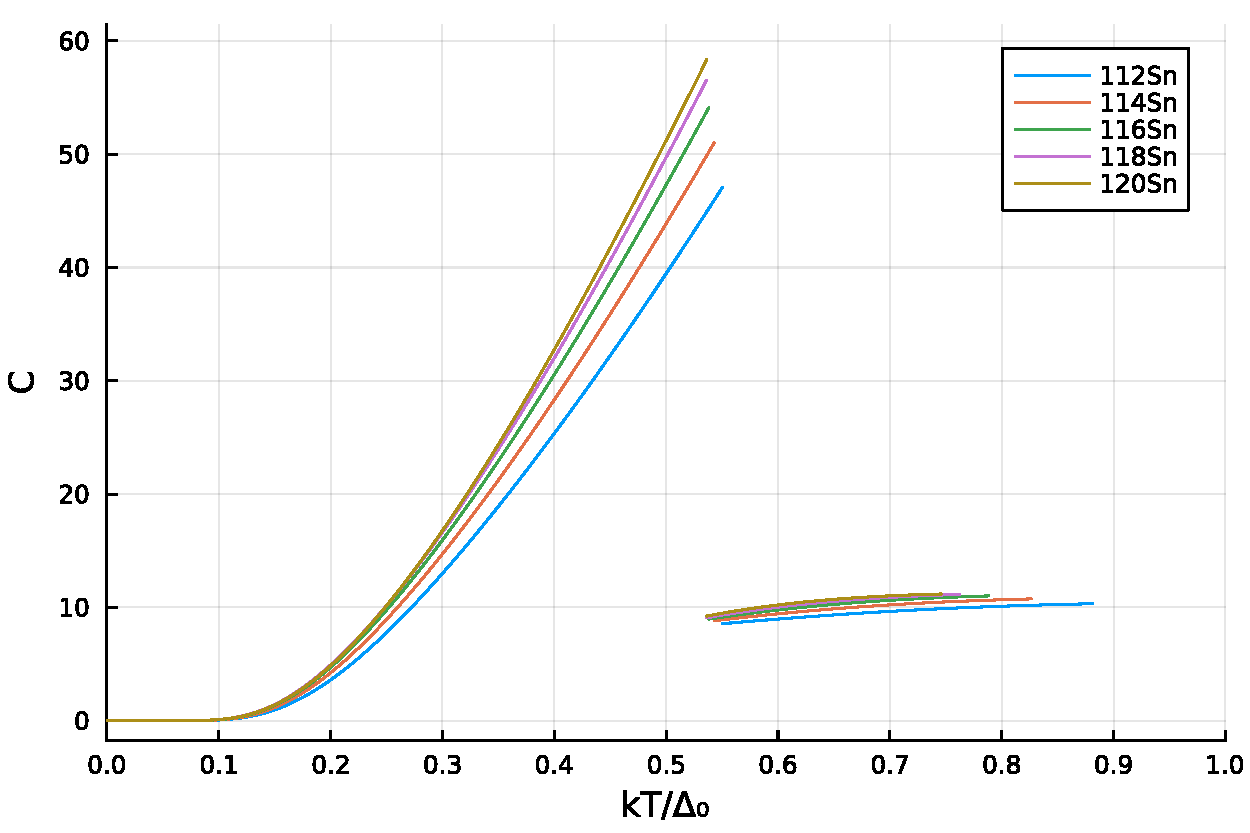
\includegraphics[width=0.65\textwidth]{main_fig/112C.pdf}
    \caption{\ce{{}^{112-120}}Snの中性子についての計算結果。上からpairing gap、エネルギー期待値、比熱に対する温度変化。}
  \end{figure}
  \newpage
  \begin{figure}[H]
    \centering
    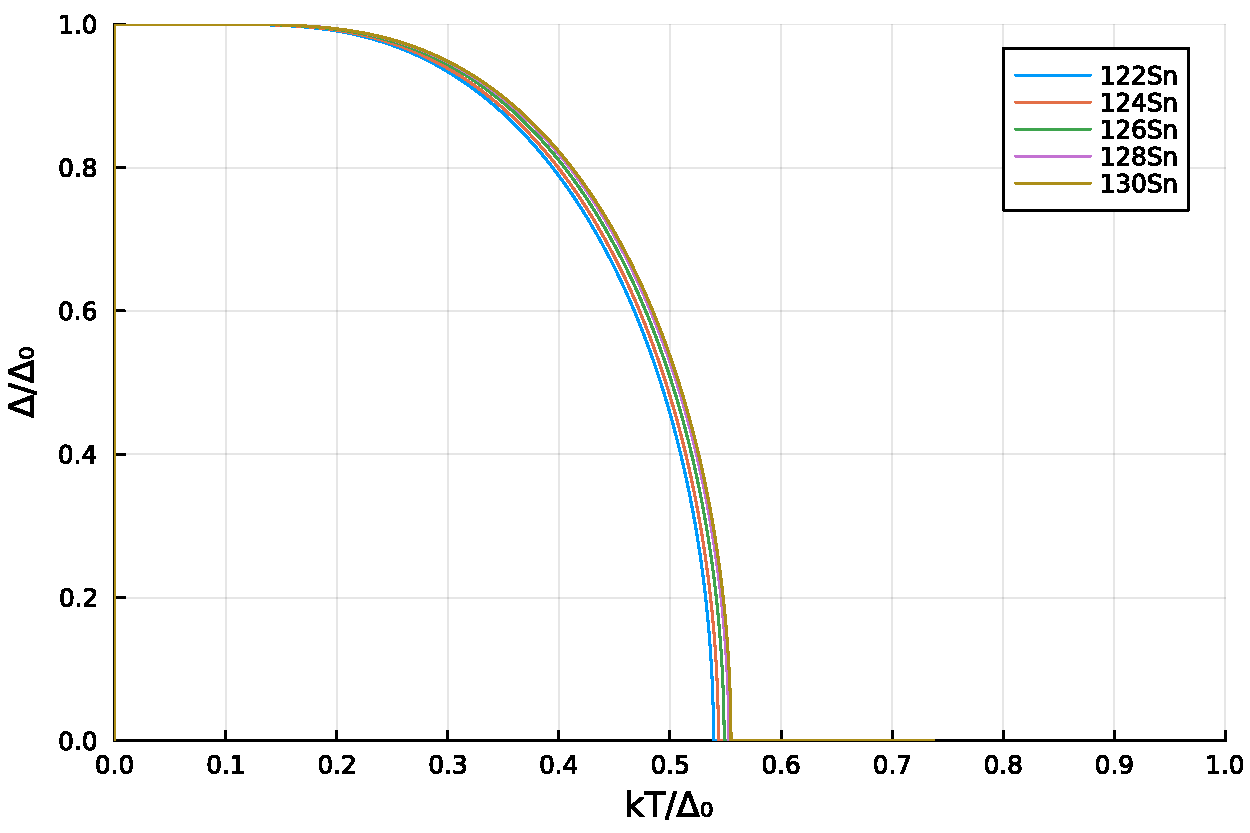
\includegraphics[width=0.65\textwidth]{main_fig/122d.pdf}
    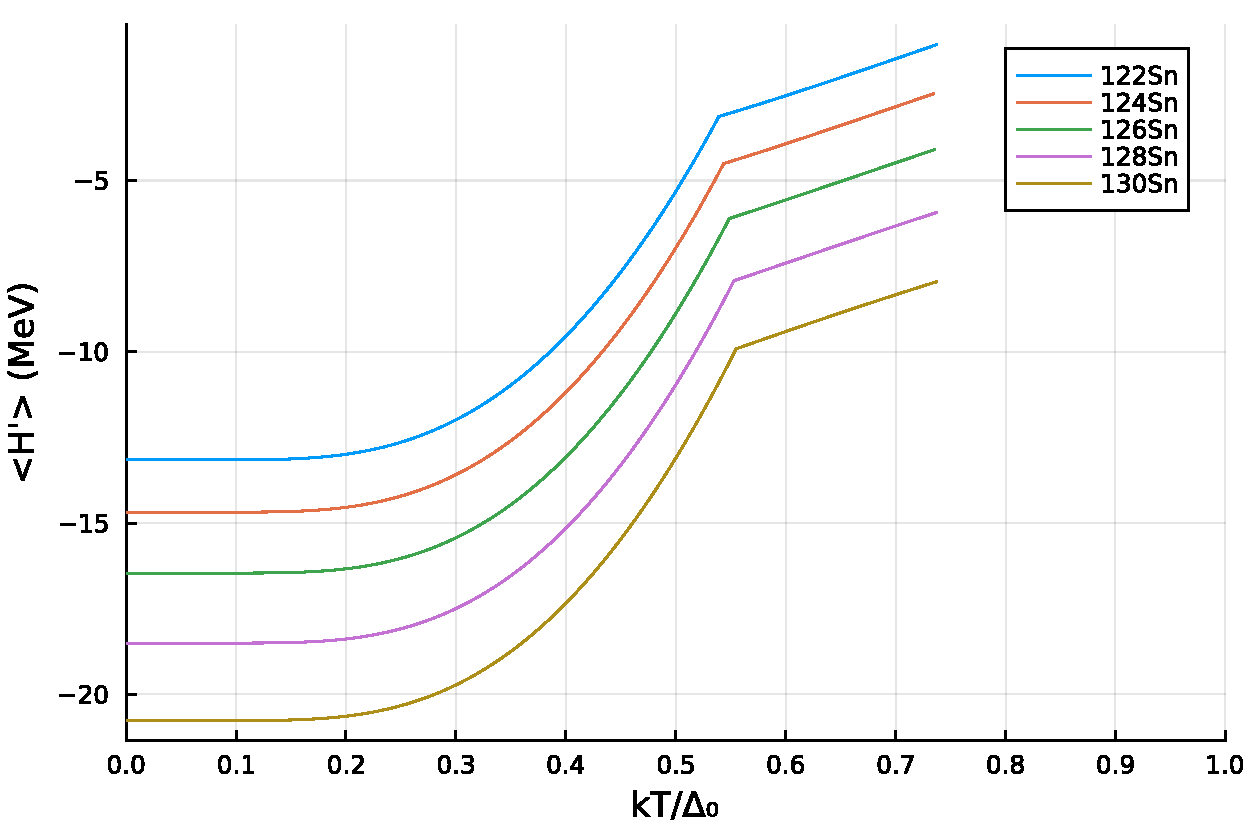
\includegraphics[width=0.65\textwidth]{main_fig/122H.pdf}
    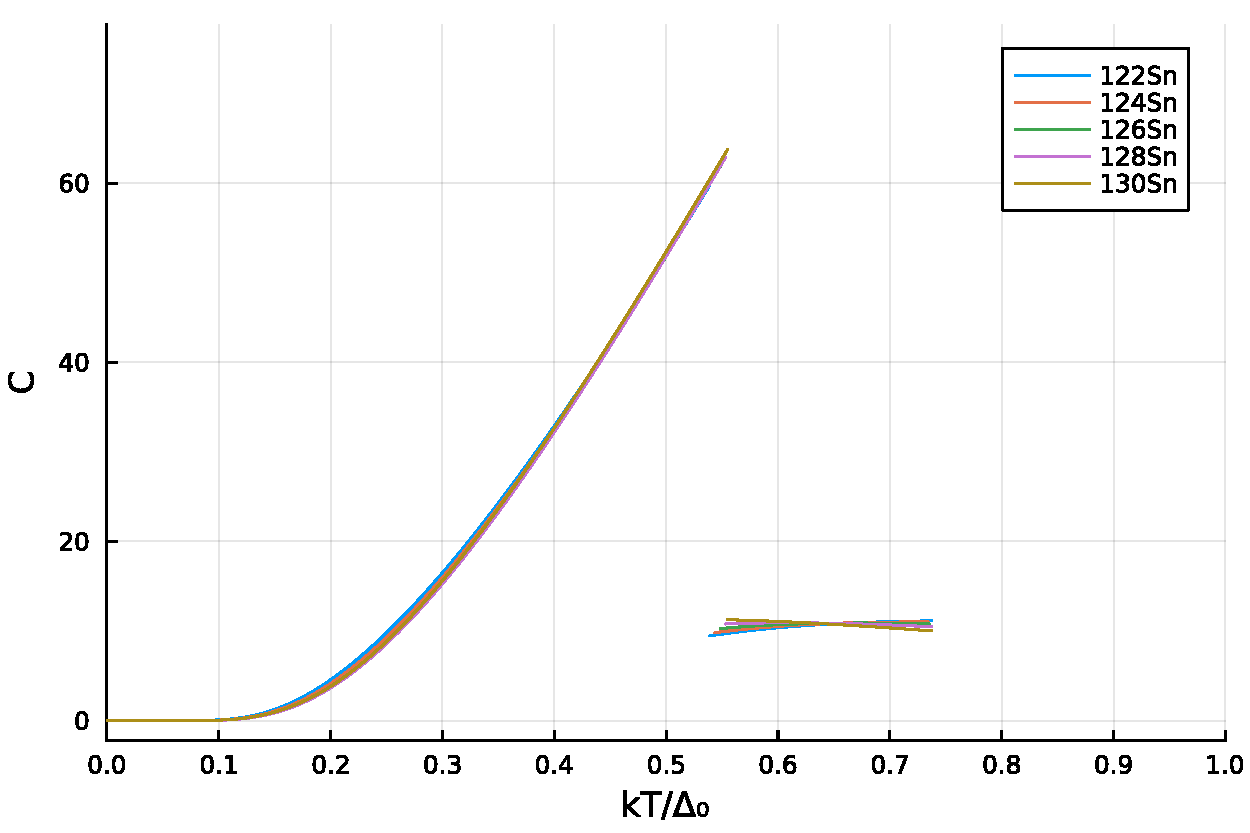
\includegraphics[width=0.65\textwidth]{main_fig/122C.pdf}
    \caption{\ce{{}^{122-130}}Snの中性子についての計算結果。上からpairing gap、エネルギー期待値、比熱に対する温度変化。}
  \end{figure}
  \begin{table}[H]
    \centering
    \caption{核子数と相転移温度の対応表}
    \label{tab:transition_temperature}
    \begin{tabular}{cccccc}
        \toprule
        核子数 & $k_B T_c$ (MeV) & 核子数 & $k_B T_c$ (MeV) & 核子数 & $k_B T_c$ (MeV) \\
        \midrule
        102 & 0.30535 & 112 & 0.62420 & 122 & 0.73118 \\
        104 & 0.39563 & 114 & 0.65673 & 124 & 0.74009 \\
        106 & 0.47009 & 116 & 0.68266 & 126 & 0.74631 \\
        108 & 0.53269 & 118 & 0.70309 & 128 & 0.75035 \\
        110 & 0.58351 & 120 & 0.71904 & 130 & 0.75242 \\
        \bottomrule
    \end{tabular}
  \end{table}
  \begin{figure}[H]
    \centering
    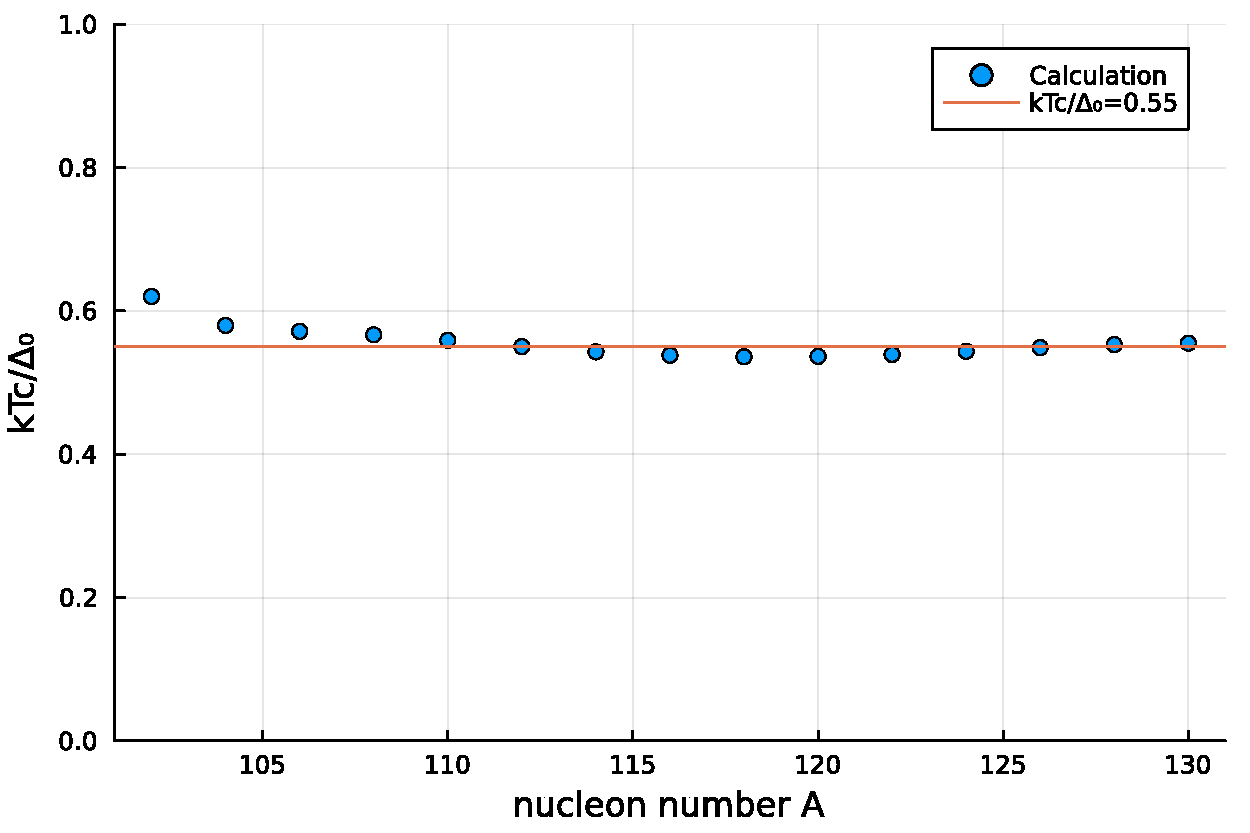
\includegraphics[width=0.8\textwidth]{main_fig/kTc_vs_A.pdf}
    \caption{核子数 $A$ に対する相転移温度 $k_B T_c$ の依存性を示すプロット。水平線 $k_B T_c/\Delta_0 = 0.55$ MeV は相転移温度の傾向を表す。}
  \end{figure}
  
  計算結果として、すべての各種において温度変化により\(\Delta=0\)になる相転移が確認できた。
  加えて、$k_B T_c/\Delta_0\simeq0.55$の傾向が見られる。
  ここで、$\Delta_0=12A^{-1/2}$であるから、核子数を指定すれば相転移温度が予想できるという結果が得られた。
  これはBCS理論の文献(有本\cite{arimoto})の、\(k_BT_c/\Delta_0=0.566\)と近い値が得られた。
  \ce{{}^{102}Sn}については、少し傾向から外れているものの許容範囲であると考える。
  この相転移は高温領域においてはpairingの崩壊により、相転移が発生した。
  pairing gap以外の物理量においても相転移温度付近での急激な変化が確認できた。

  % 結論
\chapter{結論}
  \section{本研究のまとめ}
  本研究では、100〜130Sn核を対象に、有限温度における超流動から常流動への相転移を解析した。  
  そのために、Woods-Saxonポテンシャルとseniorityペアリングモデルを用いたハミルトニアンを構築し、  
  BCS理論およびその有限温度拡張を適用して数値計算を行った。

  本研究の主要な結果は以下の通りである:
  \begin{enumerate}
      \item 化学ポテンシャルの振る舞いについて、核子数に対して単調に増加することが確認された。
      \item 近似式と比較した結果、計算結果の傾向は一致しており、Woods-Saxonポテンシャルとseniorityペアリングモデルの適用が妥当であることが示された。
      \item すべての計算対象核において、温度上昇に伴いペアリングギャップ $\Delta$ が消失する相転移が確認された。
      \item 相転移温度 $T_c$ に関して、$k_B T_c/\Delta_0 \simeq 0.55$ の関係が得られ、BCS理論の既存研究(有本\cite{arimoto})で示されている $k_B T_c/\Delta_0=0.566$ に近い値を示した。
      \item すべての核種でギャップ消失(超流動から常流動への相転移)が発生し、ギャップ以外の物理量(エネルギー期待値、比熱)においても相転移温度付近での急激な変化が確認された。
  \end{enumerate}

  これらの結果は、102〜130Sn核における超流動状態の有限温度での振る舞いを明らかにするものであった。
  \section{今後の課題}
  今回の解析では、有限温度においても平均場ポテンシャルを変化させなかった。
  そのため、詳細な有限温度の解析が行われていないと想定されるため、有限温度の平均場近似を行うことは有意義である。
  加えて、BCS理論によって破れた対称性を回復するために粒子数射影、角運動量射影を行うことによる発展も考えられる。

% 参考文献
\bibliographystyle{junsrt}
\bibliography{list} % BibTeXファイルを使う場合

% 付録(必要なら)
\appendix
\chapter{有限温度BCS理論の詳細な導出}\label{FTBCS導出}
  grand canonical分布を用いて平衡状態を考える。(温度$T$,化学ポテンシャル$\mu$はConst.)
  
  グランドポテンシャル$\Omega=E- TS -\mu N$から変分法を用いて
  密度op.$D$を定義し、$\operatorname{Tr}D=1$という性質で、これを用いれば分配関数と密度演算子
  は以下のように決められる。
  \begin{align}
    D &= Z^{-1}e^{-\beta(H-\mu N)}\\
    Z &= \operatorname{Tr}\left[e^{-\beta(H-\mu N)}\right]
  \end{align}
  また演算子$O$の期待値は、
  \begin{equation}
    \left\langle O\right\rangle=\operatorname{Tr}DO\label{期待値}
  \end{equation}
  である。
  これがHFB近似のもとではquasi-particle Hamiltonian\ $\operatorname{H_{\text{HFB}}}$が
  quasi-particle 真空エネルギー$E_0$,quasi-particle エネルギー$E_i$,
  quasi-particle creation op.$a_i^{\dagger}$を使って
  $\operatorname{H_{\text{HFB}}}=E_0 + \sum_{i}E_i a_i^{\dagger}a_i$
  と表すことができることから、HFB 密度演算子とHFB分配関数は
  \begin{align}
    D_{\text{HFB}} &= Z_{\text{HFB}}^{-1}\exp\left(-\beta \sum_i E_i \hat{n}_i\right)\\
    Z_{\text{HFB}} &= \operatorname{Tr}\left[\exp\left(-\beta \sum_i E_i \hat{n}_i\right)\right]
  \end{align}
  ただし、$\hat{n}_i = a_i^{\dagger}a_i$。
  この分配関数を展開すれば、
  \begin{align}
    Z_{\text{HFB}} &= \operatorname{Tr}\left[\exp\left(-\beta \sum_i E_i \hat{n}_i\right)\right]\\
    &= \sum_{n_i}\prod _{i} e^{-\beta E_i n_i}
  \end{align}
  となるが、quasi-particle近似において$n_i=0,1$であるから、$\hat{n}_i^2=\hat{n}_i$より、
  \begin{equation}
    Z=\prod _{i} \left(1 + e^{-\beta E_i}\right)
  \end{equation}
  と展開できる。
  これを使えば密度演算子は
  \begin{equation}
    D_{\text{HFB}} = Z_{\text{HFB}}^{-1}\prod _{i}
    \left[e^{-\beta E_i}\hat{n}_i + (1 - \hat{n}_i)\right]
  \end{equation}
  となる。ここは$n_i=0,1$を主に用いた。Fermi分布関数$f_i=1/(1 + e^{\beta E_i})$を使えば、
  \begin{equation}
    D_{\text{HFB}}=\prod_i \left[f_i\hat{n}_i+(1 - f_i)(1 - \hat{n}_i)\right]
  \end{equation}
  ここまではquasi-particleを使っていたので変換式
  $a_i^{\dagger} = \sum_{j}(U_{ij}c_j^{\dagger}+V_{ij}c_j)$から
  逆変換を行うことで単粒子の場合の密度とペアリングテンソルを求める。
  式(\ref{期待値})からそれぞれ、
  \begin{align}
    \rho_{ij} &= \langle c_j^\dagger c_i\rangle=\operatorname{Tr}D c_j^\dagger c_i\\
    t_{ij}    &= \left\langle c_j c_i\right\rangle=\operatorname{Tr}D c_j c_i
  \end{align}

  これを逆変換を行いながら
  $\bar{\rho}_{ij}=\langle a_j^\dagger a_i\rangle=\operatorname{Tr}D a_j^\dagger a_i=\delta_{ij}f_i,
  \bar{t}_{ij}=\langle a_j a_i\rangle=0$を用いて計算を進めると、
  \begin{align}
    \rho &= \tilde{U}fU^{*} + V^{\dagger}(1-f)V \\
    t    &= \tilde{U}fV^{*} + V^{\dagger}(1-f)U
  \end{align}
  のようになる。
  これは$T=0$のときに$f=0$になることから普段のBCS方程式と一致することがわかる。
  また、このときの粒子、空孔状態のエントロピー$S$と粒子数$N$は
  \begin{align}
    S &= -k\sum_{i}\left[f_i\ln f_i + (1-f_i)\ln (1 - f_i)\right]\\
    N &= \operatorname{Tr}\rho
  \end{align}
  その他の手続きは$T=0$のときとあまり変わらずに、Hamiltonianが、
  \begin{equation}
    H=\sum_{i}\epsilon_ic_i^{\dagger}c_i-\sum_{ij>0}G_{ij}c_i^{\dagger}c_{\bar{i}}^{\dagger}c_{\bar{j}}c_i
  \end{equation}
  としたときに、$E_i=E_{\bar{i}}=[(\epsilon_i -\mu)^2 +\Delta_i]^{1/2}$を用いて、
  \begin{align}
    u_i^2 = \dfrac{1}{2}(1+\epsilon_i/E_i)\\
    v_i^2 = \dfrac{1}{2}(1-\epsilon_i/E_i)
  \end{align}
  これを$U,V$に代入してペアリングテンソルを計算すれば、
  \begin{align}
    t_{i\bar{i}}=u_iv_i(1-2f_i)\\
    u_iv_i=-\dfrac{\Delta_i}{2E_i}\\
    1-2f_i=\tanh(1/2\beta E_i)
  \end{align}
  よってgap方程式は$\Delta_i=-\sum_{k>0}G_{ik}t_{k\bar{k}}$より、
  \begin{equation}
    \Delta = \dfrac{1}{2}\sum_{j>0}G\dfrac{\Delta}{E_j} \tanh{(1/2\beta E_j)}
  \end{equation}
  これは$T=0$のときに$\tanh = 1$となり一致する。
\chapter{自由エネルギーとエントロピーの温度変化}
  \vspace{-10pt}
  エントロピー\(S = -k_B \sum_{k}\left[f_k \ln f_k +(1 -f_k)\ln (1-f_k) \right]\)と
  自由エネルギー\(F=H-TS\)
  の計算結果を\ce{{}^{116}Sn}の場合について下に示す。
  \vspace{-5pt}
  \begin{figure}[H]
    \centering
    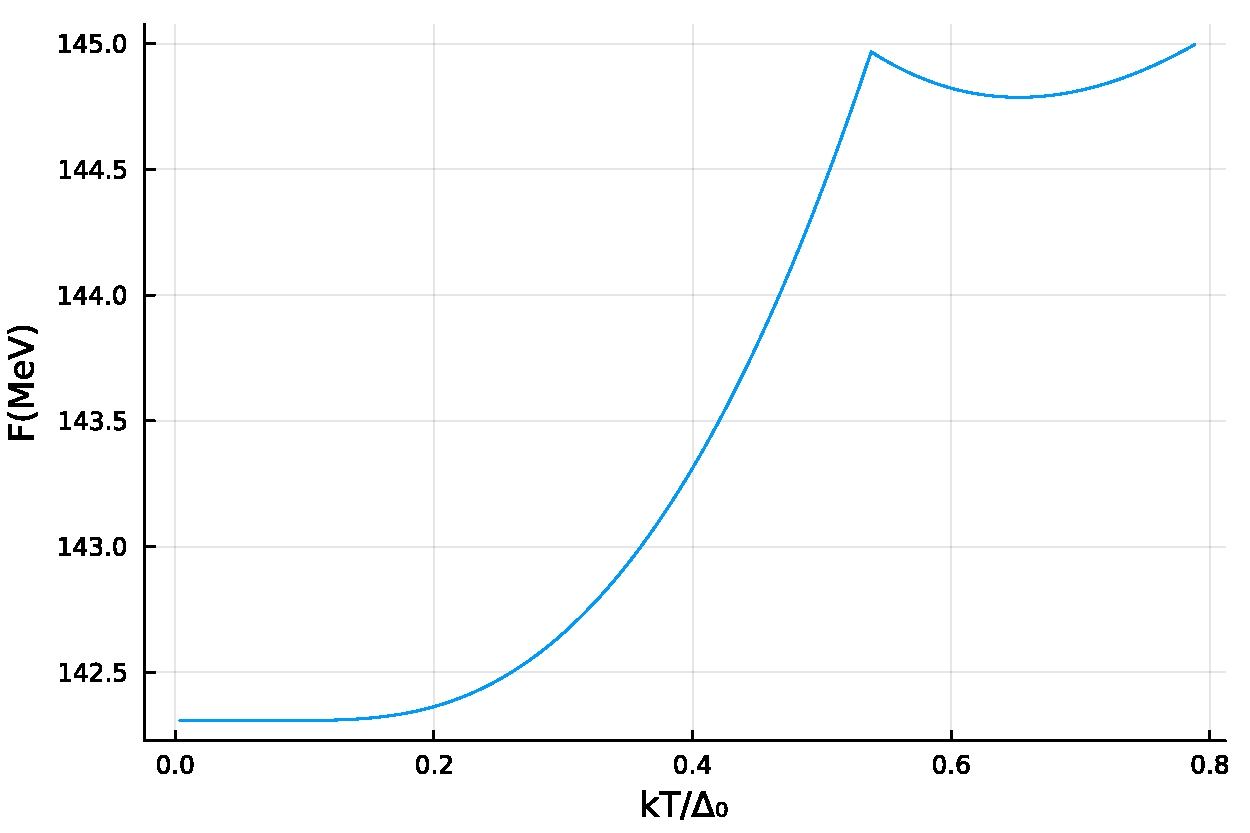
\includegraphics[width=0.7\textwidth]{main_fig/F_kT.pdf}
    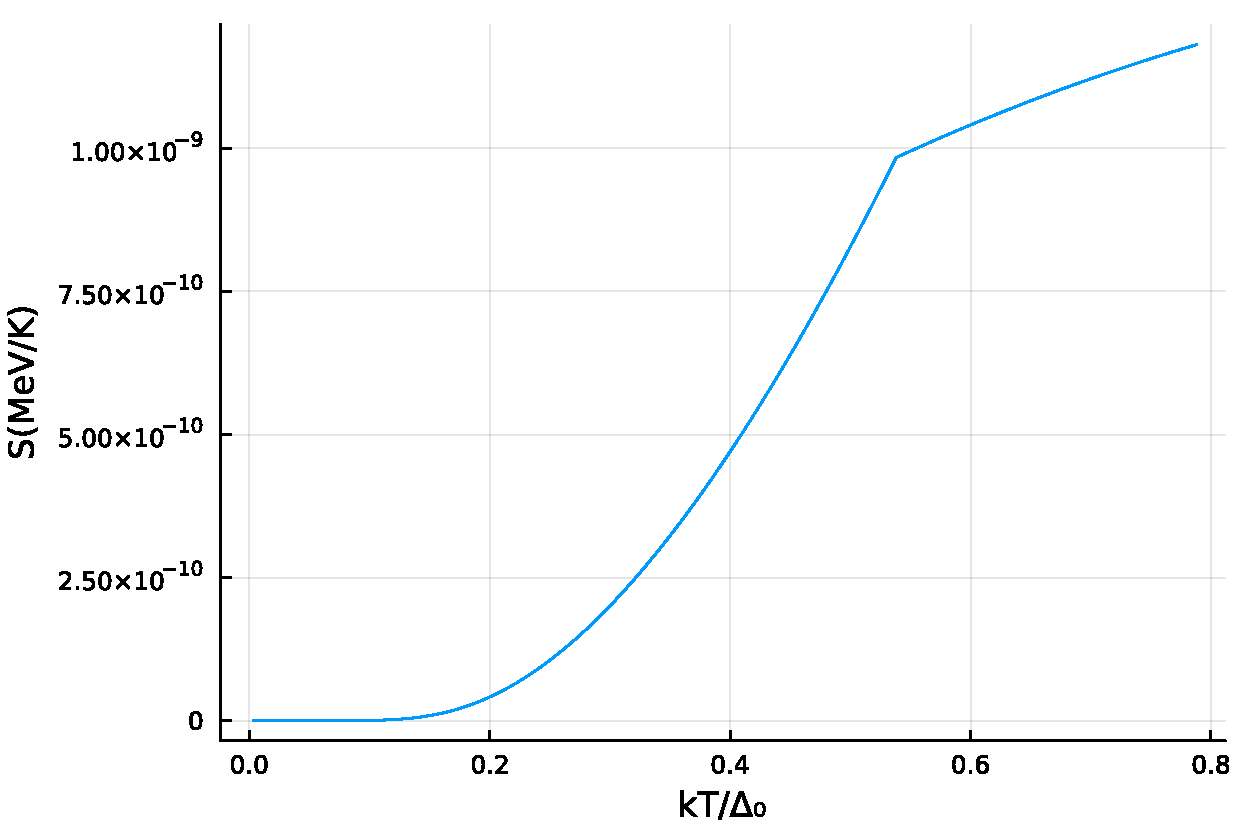
\includegraphics[width=0.7\textwidth]{main_fig/S_kT.pdf}
    \caption{116Sn核におけるエントロピー $S$ および自由エネルギー $F$ の温度依存性。}
  \end{figure}



\end{document}
